%% This LaTeX-file was created by <rw7> Sat Apr 28 21:25:42 2001
%% LyX 0.12 (C) 1995-1998 by Matthias Ettrich and the LyX Team

%% Do not edit this file unless you know what you are doing.
\documentclass[a4paper,english]{report}
\usepackage[T1]{fontenc}
\usepackage[latin1]{inputenc}
\usepackage{babel}
\usepackage{graphics}

\makeatletter


%%%%%%%%%%%%%%%%%%%%%%%%%%%%%% LyX specific LaTeX commands.
\newcommand{\LyX}{L\kern-.1667em\lower.25em\hbox{Y}\kern-.125emX\spacefactor1000}

%%%%%%%%%%%%%%%%%%%%%%%%%%%%%% Textclass specific LaTeX commands.
\newenvironment{lyxcode}
  {\begin{list}{}{
    \setlength{\rightmargin}{\leftmargin}
    \raggedright
    \setlength{\itemsep}{0pt}
    \setlength{\parsep}{0pt}
    \ttfamily}%
   \item[]}
  {\end{list}}

%%%%%%%%%%%%%%%%%%%%%%%%%%%%%% User specified LaTeX commands.
\usepackage{textcomp}
\makeatother

\begin{document}


\title{Diploma Thesis:\\
Utility Support for Checking OCL Business Rules in Java Programs}


\author{Ralf Wiebicke}


\date{December 2000}

\maketitle
\cleardoublepage


\section*{Copyright}

Copyright \copyright~2000 Ralf Wiebicke.

Permission is granted to copy, distribute and/or modify this document under
the terms of the GNU Free Documentation License, Version 1.1 or any later version
published by the Free Software Foundation; with no Invariant Sections, no Front-Cover
Texts, and no Back-Cover Texts. A copy of the license is available at http://www.gnu.org/copyleft/fdl.html.

The source code developed together with this paper is Copyright \copyright~2000
Ralf Wiebicke and published under the GNU Lesser General Public License (LGPL).
Additional source code was developed by Steffen Zschaler under LGPL.


\section*{Availability}

This document is available at http://rw7.de/ralf/diplom00/intro.html in several
electronic forms including \LaTeX{}, Postscript, PDF, HTML and the original
k\LyX{} version.

The source code developed together with this paper is available at http:// dresden-ocl.sourceforge.net/.


\section*{Modifications}

This version includes several post-submission updates as listed below. For the
submission version see the CVS repository.

\begin{itemize}
\item The paper moved to http://rw7.de/ralf/diplom00/intro.html.
\item Versant provided a fix for the bug mentioned in chapter\ref{Sec:chapterIndustrial}
and appendix\ref{sec: VersantProblem}.
\item Removed \texttt{-{}-xmi-model} in \ref{Sec:UsageReference}, was superfluous
and caused some trouble.
\end{itemize}
\cleardoublepage

\tableofcontents

\cleardoublepage


\chapter{Introduction}

This work describes the design and implementation of runtime verification of
OCL (Object Constraint Language) constraints in java programs. Therefore, the
OCL compiler developed by Frank Finger \cite{ff3} was extended into a java
source code instrumentation tool. 


\section{Motivation}

Many different approaches for increasing software quality have been developed
in the past. Few of them have experienced wide spread usage in industry. One
of them is Structural Programming, another one is the Object Oriented Paradigm.
And there is just another one, which convinces through its simpleness: Check
Statements (or \texttt{assert}ions in C++).

Suppose a method for removing all objects from a collection:

\begin{lyxcode}
void~clear()

\{

~~//~some~complex~handling~of~

~~//~hash~tables~or~trees~...

\}
\end{lyxcode}
Now, how does one verify, that the (supposedly complex) implementation is correct?
Starting up the debugger and check for a few cases? Is Russian Roulette. Building
some automatic test cases? Getting better. But why not make sure, that the critical
code works correctly for the rest of its life:

\begin{lyxcode}
void~clear()

\{

~~//~some~complex~handling~of~

~~//~hash~tables~or~trees~...

~~assert(size()==0)

\}
\end{lyxcode}
The \texttt{assert} statement terminates the program, if the given expression
evaluates to false. Otherwise it does nothing. Many bugs would be detected when
showing up for the first time\footnote{
The rare case, where a bug in \texttt{size()} happens to hide a bug in \texttt{clear()}
is neglected here.
}. Additionally it needs only a compiler switch to disable all assertions, thus
removing any runtime penalty for release versions. As described in \cite{bugs},
software quality can be improved dramatically by using assertions whenever possible.
This meets with practical experiences of the author.

Unfortunately, there is no \texttt{assert} statement in Java. A similar functionality
could be achieved using exceptions, but there would be no possibility to globally
disable assertions.

Furthermore, assertions are just a special case of a much more powerful concept:
Design by Contract (DbC). A good introduction is given in \cite{DbC}. In DbC
the example assertion above is transformed into a postcondition of the method:

\begin{lyxcode}
/{*}{*}

~~~@postcondition:~size()==0

{*}/

void~clear()

\{

~~//~some~complex~handling~of~

~~//~hash~tables~or~trees~...

\}
\end{lyxcode}
The tool developed with this paper aims to support verification of design constraints
as shown above. It instruments java source code, so that the instrumented code
checks its own constraints on runtime. 


\section{Task}

This work aims to extend the OCL compiler developed by Frank Finger with a java
source code instrumentation tool. \cite{ff3} section 3.6 already provides a
list of requirements for such a tool. Additional attention is paid to java programs,
where no UML class diagrams are available. The tool should be implemented to
a sufficient extent. This includes maintance of the existing OCL compiler. For
the java code provided by the industrial partner, net-linx AG, a small set of
typical OCL constraints will be developed and experimented with.


\section{Organisation of This Work}

Chapter \ref{Sec:chapterRelated} lists work related to this paper, particularly
software aiming for similar functionality. Chapters \ref{Sec:chapterCodeInjection}
and \ref{Sec:chapterModelInformation} present the design and implementation
of the two major extensions of the OCL compiler developed in this paper: the
java source code instrumentation and the completed model information for OCL.
Chapter \ref{Sec:chapterIndustrial} reports experiences made using the tool
on an industrial strength project. Chapter \ref{Sec:chapterSummary} summarizes
the results of this work, while chapter \ref{Sec:chapterOutlook} points out
directions for future work.

Appendix \ref{Sec:chapterMaintance} lists all modifications of the OCL compiler
made during this work. Appendix \ref{Sec:chapterUsage} contains a short manual
of the software together with an illustrative example. Finally, some very detailed
descriptions have been shifted into appendix \ref{Sec:chapterCodeExamples}
to keep the main text clear.

This work comes with a CD, containing a current snapshot of the developed software,
an electronic version of this paper and software and literature referred to
in this work, where available.

\cleardoublepage


\chapter{Related Work\label{Sec:chapterRelated}}

This chapter lists both papers and software related to this diploma thesis.
For some of the work there is a detailed comparison in subsequent chapters. 


\section{Runtime Constraint Checking \label{Sec:relatedConstraints}}

This section lists tools, which perform runtime constraint checking on java
programs, more or less similar to the tool developed in chapter \ref{Sec:chapterCodeInjection}. 

JMSAssert (\cite{JMSAssert}) provides OCL support for java. Constraints are
embedded into javadoc comments. The tool links into the JVM to make the constraints
checked. This approach does not involve source code modification. This makes
it easier to use, but also platform dependent (currently Windows only). It also
requires just-in-time compilers to be switched off. Binaries are available at
no cost.

Several approaches instrument java byte code to make constraints checked, such
as Handshake (\cite{Handshake}) and jContractor (\cite{jContractor}). Section
\ref{sec: compareByteCodeInstr} discusses, whether the approach of source code
instrumentation presented in this paper is adaptable to byte code instrumentation.
Handshake uses separate text files with a non-standard syntax to express class
invariants and pre/postconditions. jContractor implements constraints with dedicated
java methods. Neither Handshake nor jContractor binaries are publicly available.

iContract (\cite{iContract}) is a preprocessor for java. It instruments java
source code to check constraints. It supports a subset of OCL. Constraints are
embedded into javadoc comments. iContracts source code instrumentation is analyzed
in detail in section \ref{sec: compareIContract}. Binaries are available at
no cost.

For some applications OCL is just too powerful. A simpler approach is demonstrated
in \cite{kbeans}. It implements a number of predefined constraint types, such
as \emph{numeric range} or \emph{ordering of arrays}. For instance to have an
attribute \texttt{age} constrained to positive values, one just adds a method
\texttt{getAge\-Min\-Value()~\{return~0;\}}. Most OCL constraints used in
the development of the OCL toolkit also could have been expressed with such
simple means. Constrained classes must be valid JavaBeans. Also, the class must
announce the modification of attributes manually to have the constraints reevaluated.
KBeans is released under GPL. Additionally there is a GUI for simulating an
object population and checking constraints against it.

Jass (\cite{jassWeb}) is a preprocessor for java assertions developed at the
University of Oldenburg (\cite{jassDiplom}). Apart from class invariants and
method pre- and postconditions it provides check statements (like assert() in
C++) and loop invariants and variants. Assertions are expressed in java, extended
by universal and existential quantifiers. Section \ref{sec: compareJass} analyses
the code instrumentation of Jass in detail. Jass is available under GPL.

The following table summarizes the tools introduced above. The last line shows
the tool developed with this paper.

\vspace{0.3cm}
{\centering \begin{tabular}{|c||c|c|c|}
\hline 
&
Constraint Source&
Verification Method&
Availability\\
\hline 
\hline 
JMSAssert&
OCL in javadoc&
links JVM &
binary\\
&
&
(platform dependent)&
\\
\hline 
Handshake&
proprietary language&
byte code instr. / &
not\\
&
&
 proxy system library&
available\\
\hline 
jContractor&
 java methods&
 byte code instr. /&
not\\
&
&
class loader&
available\\
\hline 
iContract&
OCL in javadoc&
source code instr.&
binary\\
\hline 
KBeans&
predefined constraint&
in special environment&
GPL\\
&
types / java methods&
&
\\
\hline 
Jass&
java fragments in javadoc&
source code instr.&
GPL\\
\hline 
Dresden &
OCL in javadoc&
source code instr.&
LGPL\\
Toolkit&
&
(reversible)&
\\
\hline 
\end{tabular}\par}
\vspace{0.3cm}


\section{Reverse Engineering\label{Sec:relatedReverse}}

This section lists work related to reverse engineering needed in chapter \ref{Sec:chapterModelInformation}.

A powerful approach to reverse engineering has been developed at the MIT \cite{womble}.
The tool Superwomble extracts an object model from java byte code. Object models
are roughly a subset of UML class diagrams, featuring inheritance and object
associations. An important challenge for the analysis is the detection of element
types of container attributes. The tool performs this very efficiently, without
requiring any additional help from the user. Thus, it complements the two approaches
presented in this paper. A detailed comparison is provided in section \ref{Sec:ReverseEngineering}.

JVision \cite{jvision} produces class diagrams from java source or byte code.
It's easy to use and has nice auto-layout. But it does not handle associations
in any way. Collection attributes are simply shown as attributes. Instead it
analyses, which classes instantiate/use each other. This is not nearly as useful
as associations.


\section{Other Related Work}

Cybernetic Intelligence develops an OCL compiler (\cite{Cybernetic}). The current
prototype claims to support syntax checking only. Type checking is under development.
Frontends are available for Select Enterprise and Rational Rose.

Elixir (\cite{elixir}) claims OCL support in it's CASE tool and its java IDE.
The CASE tool provides an OCL text field only, without any syntax checking.
For the IDE a plugin is provided to integrate iContract.

Several approaches implement OCL upon object repositories, such as USE \cite{USE}
and ModelRun \cite{Bold}. The object repositories can be populated and animated
visually, with OCL constraints continuesly being checked.

There is a universal code instrumentation toolkit (\cite{CodeInstrumentation})
available for java. It parses java files into parse trees, preserving white
space and comments. The parse tree can be modified and written back into the
file. There are various applications for this, including tracing/profiling of
program execution. The code instrumentation developed in this paper could probably
be realized using this toolkit. However, the parser analyses the complete java
file, thus is much more heavy-weight than the parser developed with this paper.
There is a test version available at no cost, limited in the size of source
programs it can handle.

\cleardoublepage


\chapter{Code Instrumentation \label{Sec:chapterCodeInjection}}

Insertion of generated code into java programs is the main subject of this paper.
Such an automatic source code transformation is commonly referred to as code
instrumentation. In this paper it covers anything beyond code generation, to
get a java program checking its own constraints. For an idea, where code generation
ends and instrumentation starts, see section \ref{Sec:codegeneration_result}. 

This is followed by an analysis of requirements for the code instrumentation
and resulting design decisions in section \ref{Sec:injection_requirements}.
Section \ref{Sec:wrappingMethods} describes the solution in detail. 

Finally sections \ref{Sec:temporalScope} and \ref{Sec:structuralScope} discuss
the more fundamental issue, when and how often invariants have to be checked.


\section{Results of Code Generation\label{Sec:codegeneration_result}}

The java code generator developed in \cite{ff3} produces a set of code fragments\footnote{
see documentation of class \texttt{tudresden.ocl.codegen.CodeFragment.}
}. These code fragments have the following properties:

\vspace{0.3cm}
{\centering \begin{tabular}{|l|p{70mm}|}
\hline 
Property &
\\
\hline 
\hline 
Constrained~type &
The class this constraint applies to.\\
\hline 
Kind &
Specifies, whether this fragment is an invariant, a pre- or a postcondition
or a transfer or preparation fragment for a postcondition. \\
\hline 
Constrained~operation &
The operation, this constraint applies to (not valid for invariants).\\
\hline 
Code &
Contains the actual java code to be executed.\\
\hline 
Result~variable &
Specifies the name of the boolean variable, which contains the result of the
OCL expression after code execution.\\
\hline 
\end{tabular}\par}
\vspace{0.3cm}

For each postcondition containing a @pre expression there are two additional
code fragments called preparation and transfer. See below.


\subsection{Preparation and Transfer Fragments}

The meaning of preparation and transfer fragments is explained on a dramatically
simplified example. 

Suppose a post condition for operation \texttt{employ()}, that leaves the attribute
\texttt{age} unchanged:

\begin{lyxcode}
context~Person::employ()~\\
post:~age=age@pre
\end{lyxcode}
The following code fragments will be produced:

\vspace{0.3cm}
{\centering \begin{tabular}{ll}
\hline 
Kind&
 Code\\
\hline 
\hline 
Transfer&
\texttt{int~node1;} \\
\hline 
Preparation&
\texttt{node1=this.age;}\\
\hline 
Post Condition&
\texttt{int~node2=this.age;}\\
&
\texttt{boolean~result=(node1==node2);}\\
\hline 
\end{tabular}\par}
\vspace{0.3cm}

Typically these fragments would be inserted as follows:

\begin{lyxcode}
class~Person\\
\{\\
~~void~employ()\\
~~\{\\
~~~~int~node1;~~~~~~~//~transfer~fragment\\
~~~~node1=this.age;~~//~preparation~fragment\\
~~~~//~original~code~of~employ()\\
~~~~//~post~condition~fragment\\
~~~~node2=this.age;\\
~~~~boolean~result=(node1==node2);\\
~~\}\\
\}
\end{lyxcode}
Note, that precise semantics of code fragments involving the @pre expression
has been changed, so that the original meaning described in \cite{ff3} section
7.1.2 is no longer fully correct. For a detailed comparison see section \ref{Sec:maintainJavaCodeGenerator}.

\begin{lyxcode}
~
\end{lyxcode}

\section{Requirements and Design Decisions\label{Sec:injection_requirements}}

This section analyzes the requirements for the code instrumentation and derives
some fundamental design decisions.


\subsection{Reversable Modification\label{Sec:injection_requirements_reversable}}

The most important feature is the reversability of code instrumentation. It
must be possible to

\begin{itemize}
\item clean the code tracelessly from all inserted fragments.
\item redo the instrumentation on source code that has already been modified, for
instance when constraints have been changed. 
\item edit the modified source code without losing all changes at the next instrumentation. 
\end{itemize}
These requirements makes things quite a bit more difficult, but there are serious
reasons for this. Otherwise there would be two versions of source code: the
original and the modified version. This raises some unpleasant problems:

\begin{enumerate}
\item Configuration management must handle two source code trees.
\item Developers must be careful to edit the original version only.
\item Running the instrumentation is required after every change of the java source
code, not only when the constraints have been changed. 
\item Stack traces of runtime exceptions point to the modified source code. Developers
must look for the corresponding place in the original version.
\end{enumerate}
The implementation of reversable modification requires a strategy of minimally
invasive modification. This is realized by two design decisions:

\begin{enumerate}
\item Method wrappers, explained detailed in section \ref{Sec:wrappingMethods}.
\item Explicit package qualifiers for the OCL library in the generated code. Otherwise,
an \texttt{import} statement for the OCL library would be necessary. This would
be just another spot, were the original source code had to be touched. Additionally,
this may introduce name conflicts between OCL library and user code.
\end{enumerate}

\subsection{Embedding Constraints in Java Source Code.\label{Sec:embedConstraints}}

It should be possible to embed constraints in the javadoc comments. The placement
of embedded constraints implicates (and replaces) the context of the constraint.
See the example below.

\begin{lyxcode}
/{*}{*}\\
~~~@invariant~ageGreaterZero:~age>0\\
{*}/\\
class~Person\\
\{\\
~~int~age;\\
~\\
~~/{*}{*}\\
~~~~~@postcondition:~age=age@pre\\
~~{*}/\\
~~void~employ();\\
\}
\end{lyxcode}
Constraints should be immediately visible to the editor of a java file. Also,
this generally promotes the single source approach. The author is strongly convinced,
that constraints stored in an extra text file are too far away from attention.

Invariants may also be placed on an attribute or method of their context class.
This is for convenience, since most invariants are clearly related to one specific
attribute or method.


\subsection{Checking the Element Type.}

The instrumented code must check, that container attributes comply to the \texttt{@element-type}
and \texttt{@key-type} javadoc tags. For collections the \texttt{@element-type}
tag specifies the type of the objects allowed in the collection. For maps \texttt{@element-type}
specifies the type of values, while \texttt{@key-type} defines the type of key
objects. A detailed description is provided in section \ref{Sec:element_type_tag}. 

Note, that this feature may be used standalone, without OCL expressions at all.
Then it provides a runtime check for typed collections.


\section{Code Insertion\label{Sec:wrappingMethods}}

The main task of code instrumentation is to have some code executed immediately
before and after all methods (and after all constructors too). This section
describes, how this is done by the tool developed with this paper.

At first, section \ref{sec: SimpleApproach} intoduces a simple approach, and
why this would not work. Sections \ref{Sec:wrappingMethodsSub} and \ref{Sec:wrappingConstructors}
explain the approach followed in this work. A somewhat tricky caveat and how
it is solved is worked out in \ref{Sec:WrapperLoop}. Section \ref{Sec:cleaningCode}
shows, how it is managed to undo all modifications of the instrumentation. The
java parser used to do all this is outlined in \ref{sec: JavaParser}.

Sections \ref{sec: compareJass}, \ref{sec: compareIContract} and \ref{sec: compareByteCodeInstr}
compare this solution to three other tools approaching a similar task quite
differently. This is summarized in \ref{Sec:CodeInsertionSummary}.


\subsection{A Simple Approach\label{sec: SimpleApproach}}

A straight-forward solution would insert the code directly into the method.
Consider the following method.

\begin{lyxcode}
int~someMethod(double~x)\\
\{\\
~~//~here~comes~the~code.\\
~~return~result;\\
\}~
\end{lyxcode}
The generated code could be inserted like this:

\begin{lyxcode}
int~someMethod(double~x)\\
\{\\
~~//~some~code~checking~invariants/preconditions.\\
~~//~here~comes~the~code.\\
~~//~some~code~checking~invariants/postconditions.\\
~~return~result;\\
\}~
\end{lyxcode}
But this raises some severe problems:

\begin{enumerate}
\item The code to be executed after the method (postcondition and invariants) has
to be inserted before any return statement.
\item The post condition code must have the return value available. Instead of the
\texttt{result} variable in the example above, there could be a complex expression.
Such a return expression has to be computed in advance, if the post condition
code refers to the return value or the return expression produces side effects.
\item There may be name conflicts between the original and the generated code, since
the generated code defines local variables.
\item For methods with return type void it must be decided, whether the post condition
code has to be inserted at the end of the method. This depends on whether the
end of the method is a reachable point of code. For the decision it needs a
complete control flow analysis of the method. Note, that if the post condition
code is wrongly inserted at the end of the method, the java compiler will fail
due to unreachable statements.
\end{enumerate}
An implementation would need a complete java parser. The following code instrumentation
would have to modify the original code at many different places and in a complicated
way. This runs contrary to the strategy of minimally invasive modification as
decided in section \ref{Sec:injection_requirements_reversable}. 

Additionally, item 4 requires much of the semantic analysis performed by a java
compiler. This makes the simple approach very hard to implement. 

Jass (\cite{jassWeb}) and iContract (\cite{iContract}) use this simple approach
and encounter all the problems mentioned above. For a detailed comparison see
sections \ref{sec: compareJass} and \ref{sec: compareIContract}.

Method wrappers solve all these problems in a nifty but simple way. This is
introduced in the following section.


\subsection{Wrapping Methods\label{Sec:wrappingMethodsSub}}

Some code tells more than thousand words, so an example is used to explain.
Consider the following method.

\begin{lyxcode}
int~someMethod(double~x)\\
\{\\
~~//~here~comes~the~code.\\
\}~
\end{lyxcode}
This is transformed into two methods.

\begin{lyxcode}
int~someMethod\_wrappedbyocl\footnote{
This is not yet the full truth, see section \ref{Sec:WrapperLoop}.
}(double~x)\\
\{\\
~~//~here~comes~the~code.\\
\}\\
~\\
int~someMethod(double~x)\\
\{\\
~~//~some~code~checking~invariants/preconditions.\\
~~int~result=someMethod\_wrappedbyocl(x);\\
~~//~some~code~checking~invariants/postconditions.\\
~~return~result;\\
\}
\end{lyxcode}
Now let's have a look back at the problems encountered for the simple approach.
None of them exist anymore. 

\begin{itemize}
\item The code to be executed after the method has to be inserted once only.
\item When the post condition code is executed, the return expression is already evaluated
and ready to use.
\item No name conflicts are possible, since user code and generated code are strictly
separated into different methods.
\item No control flow analysis is needed.
\end{itemize}
The user code is modified in a simple way: a suffix is appended to the method
name. For an implementation a very fragmentary java parser is sufficient, which
understands ``java signature level'' only. This signature level covers anything
outside of method bodies and attribute initializers. This is a very small part
of the java language and easily to be analyzed by a hand-crafted parser. See
section \ref{sec: JavaParser} how easy it is.

This kind of method wrapping still has a problem, which has been called the
``wrapper loop'' in this paper. Section \ref{Sec:WrapperLoop} shows how this
is solved.


\subsection{Wrapping Constructors\label{Sec:wrappingConstructors}}

Another transformation is used for constructors, since they cannot be renamed.
Suppose an example constructor.

\begin{lyxcode}
SomeClass(String~x)\\
\{\\
~~//~here~comes~the~code\\
\}
\end{lyxcode}
Instead of renaming, the original constructor gets an additional dummy argument.

\begin{lyxcode}
SomeClass(String~x,~Dummy\footnote{
Actually this is class \texttt{tudresden.ocl.injection.lib.WrapperDummy}.
}~oclwrapperdummy)\\
\{\\
~~//~here~comes~the~code\\
\}\\
~\\
SomeClass(String~x)\\
\{\\
~~this(x,~(Dummy)null);\\
~~//~some~code~checking~invariants.\\
\}
\end{lyxcode}
A special case occurs if a class doesn't provide any constructors. Then the
java compiler generates a default constructor as specified in \cite{JAVA} section
8.6.7. This default constructor cannot be wrapped. Instead it is replaced by
an explicit constructor with the same access modifier as the generated default
constructor would get.


\subsection{Avoiding the Wrapper Loop\label{Sec:WrapperLoop}}

Wrapping methods as described in section \ref{Sec:wrappingMethodsSub} causes
a problem for a special situation. This sections describes this situation and
provides a solution.

The critical situation is shown in the figure below:

\vspace{0.3cm}
{\centering \resizebox*{!}{5cm}{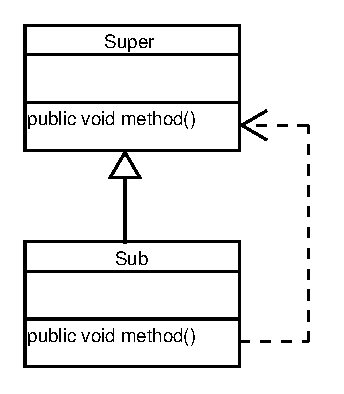
\includegraphics{WrapperLoop1.eps}} \par}
\vspace{0.3cm}

The dotted arrow represents a method call: \texttt{Sub.method()} contains a
statement \texttt{super.method();} somewhere.

The code instrumentation changes the structure as shown below:

\vspace{0.3cm}
{\centering \resizebox*{!}{5cm}{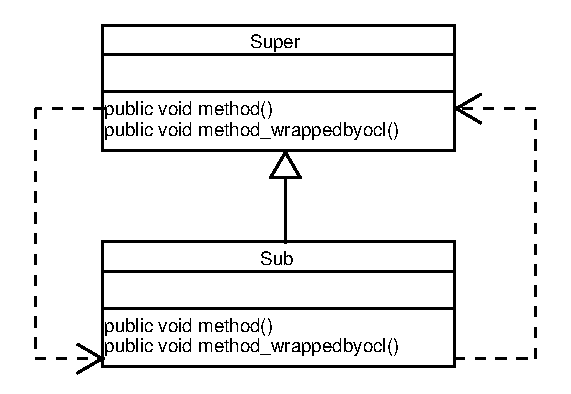
\includegraphics{WrapperLoop2.eps}} \par}
\vspace{0.3cm}

The arrows show the problem: there's an infinite loop of method calls. In detail
the following happens:

\begin{enumerate}
\item Method \texttt{Sub.method()} is called somewhere in the user program. This is
a wrapper method replacing the original method, which is named \texttt{method\_\-wrappedbyocl()}
now.
\item \texttt{Sub.method()} does some OCL specific things, before it executes the
statement \texttt{method\_\-wrappedbyocl()}. This calls the original method
\texttt{Sub.\-method\_\-wrappedbyocl()} as it is supposed to be.
\item \texttt{Sub.method\_\-wrappedbyocl()} contains the \texttt{super.\-method();}
statement, therefore calls \texttt{Super.\-method()}.
\item \texttt{Super.method()} is a wrapper method replacing the original method, which
is called \texttt{Super.\-method\_\-wrappedbyocl()} now. It does some OCL
specific thing, before it executes the statement \texttt{method\_\-wrappedbyocl()}.
But this statement does not call \texttt{Super.\-method\_\-wrappedbyocl()}
as it is supposed to be, but \texttt{Sub.method\_\-wrapped\-byocl()}, which
finally causes the infinite loop.
\end{enumerate}
The principal solution approach is simple: method \texttt{Super.\-method()}
should force \texttt{Super.\-method\_\-wrapped\-byocl()} to be executed,
although this method was overridden in class \texttt{Sub}. Java language does
not provide a way, to call a method, which was overridden. Therefore we do a
small trick:

\vspace{0.3cm}
{\centering \resizebox*{!}{5cm}{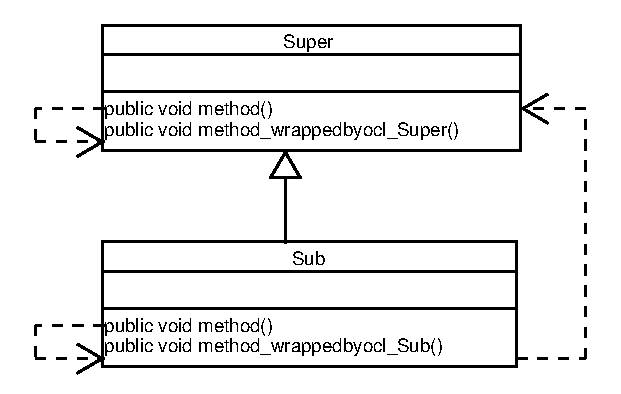
\includegraphics{WrapperLoop3.eps}} \par}
\vspace{0.3cm}

Wrapped methods get the class name appended. Thus, a wrapper method can call
the wrapped method of its own class.


\subsection{Cleaning the Code\label{Sec:cleaningCode}}

Reversable modification means, that the instrumented code can be cleaned from
any modifications without leaving any traces. This section explains, how this
requirement is met. 

The user code is modified in two different ways only:

\begin{enumerate}
\item Renaming the wrapped methods/constructors.
\item Adding new object features, e.g. wrapper methods, methods for checking invariants
and observing attributes.
\end{enumerate}
For each method to be wrapped the suffix \texttt{\_wrappedbyocl} is appended
to the name. This transformation is done on the unparsed method header, so all
typographical extras (line breaks, comments etc.) are preserved. This transformation
is easily reversed, when the code has to be cleaned. For constructors, this
works similarly with appending the dummy parameter to the parameter list.

Removing generated class features relies on the fact, that all generated features
get a special tag as shown below.

\begin{lyxcode}
/{*}{*}\\
~~~@author~ocl\_injector\\
{*}/\\
void~checkOclInvariants();
\end{lyxcode}
When cleaning the code, all object features carrying such an \texttt{@author}
tag are removed. This is quite simple and functional.


\subsection{Design of the Java Parser\label{sec: JavaParser}}

Previous sections stated, that a very simple parser is sufficient for implementing
wrapper methods. This is proven in this section by giving an overview of the
parser's design. In fact, it is as simple as a parser used for syntax highlighting
and class browsers in a java IDE.

First, the parser is actually a manipulator. The java file is simultaneously
read, parsed, modified on-the-fly and written to an output file. For a class
diagram of the parse tree produced see figure \ref{fig: JavaParser}.

\begin{figure}
{\centering \resizebox*{10cm}{!}{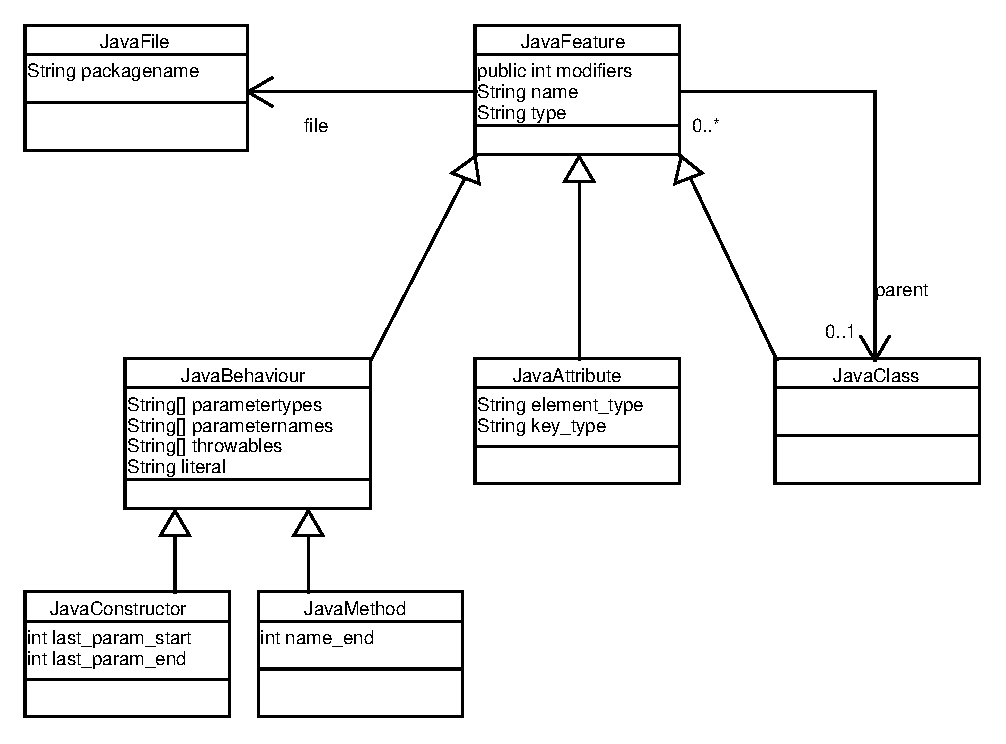
\includegraphics{JavaParser.eps}} \par}


\caption{Design of the Java Parser used by the OCL Instrumentation\label{fig: JavaParser}}
\end{figure}

The parser analyses things which are relevant for the parse tree only. Particularly
method bodies and attribute initializers are ignored. These skipped parts may
not even compile. As long as the parenthesis balance is held, the java parser
will process them correctly.


\subsection{Comparison to Jass\label{sec: compareJass}}

Jass (\cite{jassWeb}) is a precompiler for checking assertions in java programs.
It translates jass files into java. Jass files are valid java source code with
assertions specified in comments. The generated java file contains additional
code checking these assertions. Thus, Jass performs something similar to the
code instrumentation presented in the sections above. 

However, Jass directly inserts generated code into user code as described in
section \ref{sec: SimpleApproach}. Thus the problems found there should occur
in Jass too:

\begin{enumerate}
\item \emph{The code to be executed after the method has to be inserted before any
return statement.}\\
This is done by Jass. Thus, it requires a full java parser (JavaCC here).
\item \emph{The return expression has to be computed in advance.}\\
This is also done by Jass.
\item \emph{There may be name conflicts between the original and the generated code.}\\
Jass just defines a number of names (e.g. \texttt{jassResult}), which cannot
be used in the user code.
\item \emph{For methods with return type void it must be decided, whether the end
of the method is a reachable point of code.}\\
This is a known problem of Jass. It will simply fail in such cases. There is
a work around: enclose the method body into a \texttt{if(true)\{...\}} statement.
\end{enumerate}
Jass performs a complex modification of the java source code. This modification
cannot be reversed as described in section \ref{Sec:injection_requirements_reversable}.
Thus, Jass must be run before compilation whenever the source code has changed.
Additionally, the source code repository must hold jass files instead of java,
which causes administration effort for existing projects.

Jass cannot use wrapper methods, since this would not allow loop invariants
and check statements to be implemented. But without these features as in OCL,
method wrappers are much better than direct insertion of code.


\subsection{Comparison to iContract\label{sec: compareIContract}}

iContract (\cite{iContract}) is a precompiler for checking OCL constraints
in java programs. It extracts constraints from javadoc comments and produces
modified java source files checking these constraints. This is exactly the functionality,
which the tool presented in this paper tries to provide.

Just like Jass it uses direct insertion of generated code into user code. Once
again the problems found in section \ref{sec: SimpleApproach} are reviewed.

\begin{enumerate}
\item \emph{The code to be executed after the method has to be inserted before any
return statement.}\\
This has to be done by iContract. However it fails here for most cases. According
to the list of known problems \emph{``iContract generates wrong code or crashes,
if there is more than one return statement in a method.''}. This matches with
the experience of the author.
\item \emph{The return expression has to be computed in advance.}\\
This is also done by iContract.
\item \emph{There may be name conflicts between the original and the generated code.}\\
Also iContract forbids a number of names (e.g. \texttt{\_\_return\_value\_holder\_}),
to be used in the user code, although this isn't documented.
\item \emph{For methods with return type void it must be decided, whether the end
of the method is a reachable point of code.}\\
iContract doesn't do the control flow analysis needed to decide this question.
This has been proven on example in appendix \ref{sec: unreachableIConstract}.
\end{enumerate}
Experience with iContract shows, that correctly modifying java source code isn't
trivial at all. The current list of known problems suggests, that iContract
isn't usable for a real-world task. Additionally, the problem of reachable ends
of method bodies remains.


\subsection{Comparison to Byte Code Instrumentation\label{sec: compareByteCodeInstr}}

This paper is focused on source code instrumentation. Another approach is to
modify java byte code. This section discusses, whether it's possible and useful,
to apply the concept of method wrappers to byte code instrumentation.

For the third time the problems found in section \ref{sec: SimpleApproach}
are reviewed.

\begin{enumerate}
\item \emph{The code to be executed after the method has to be inserted before any
return statement.}\\
This is also needed for byte code instrumentation, but it's much easier. The
code just has to be scanned for return opcodes. 
\item \emph{The return expression has to be computed in advance.}\\
This is not needed. Whenever a return opcode is executed, the return value is
ready-to-use on the top of the execution stack.
\item \emph{There may be name conflicts between the original and the generated code.}\\
This cannot happen. Name conflicts with local variables are not possible, since
variable names do not exist anymore in byte code. Name conflicts with non-local
variables are not possible too, since they are handled by different opcodes.
\item \emph{For methods with return type void it must be decided, whether the end
of the method is a reachable point of code.}\\
This is also no problem. The java compiler takes care for it - just scan for
return opcodes. If the end of the method body isn't a reachable point of code,
then there is also no return opcode. On the other hand, if the end of a method
\emph{is} reachable, there will also be a return opcode, no matter whether there
was a return statement in the source. This is shown on example in appendix \ref{sec: byteCodeReturn},
since the JVM Specification \cite{JVM} wasn't that clear about it.
\end{enumerate}
Thus, it makes no sense, to apply the approach of method wrappers to byte code
instrumentation. 

In contrary to the approach presented in this paper, byte code instrumentation
has to be redone after every compilation of the source code. This may be done
on the fly, when loading the classes into the JVM. For instance jContractor
\cite{jContractor} uses a class loader to instrument java code. This may cause
problems, if the user code registers a class loader of it's own. This is solved
by Handshake \cite{Handshake}, which uses a proxy system library to intercept
the JVM when opening class files. Thus, Handshake buys total transparency to
the JVM with platform dependency.


\subsection{Summary\label{Sec:CodeInsertionSummary}}

Wrapping methods seems to be the best choice when instrumenting source code
for checking constraints. Several problems encountered with the simple approach
of direct insertion are solved. 

Method wrappers cannot be used, if implementation constraints (assertions, loop
invariants) are to be checked. Since OCL does not support implementation constraints,
this does not affect the scope of this paper.

Method wrappers are not useful for instrumentation on byte code level. The biggest
advantage of source instrumentation (if it is reversible) is, that it doesn't
need to be redone on each recompilation.


\section{Scope of Invariants\label{Sec:temporalScope}}

This section discusses the issue, when an constraint is required to be fulfilled.
This is trivially for pre/post conditions, but for invariants it's not so easy.

\cite{Warmer} section 5.4.2 suggests to check invariants immediately after
an object has changed\footnote{
This is partially corrected in the errata \cite{WarmerErrata}.
}. This is not workable, even if runtime efficiency is ignored. Modifications
on the model often produce intermediate states, which are not consistent according
to the constraints. 

When using databases the answer is simple: invariants must be valid outside
of transactions. Since the java system does not provide transactions there are
several strategies offered for various user requirements.

Invariants may be required to be fulfilled on:

\begin{itemize}
\item All methods. This may be too strict, since private methods may intentionally
leave an object in an inconsistent state. 
\item Public methods (or any other access modifier). This may be not strict enough.
\item Tagged methods. A special tag in the javadoc comment declares, that a method
promises to leave the system in a consistent state. This tag is then part of
the interface contract. This is the best solution, but requires additional effort
spent by the developer.
\item Explicit request. This is the way of choice, if the model is held in a database
backend. Then the checking of invariants is simply done immediately before committing.
\end{itemize}
These strategies may be used in conjunction. Except of \emph{All Methods} together
with \emph{Public Methods} and/or \emph{Tagged Methods} all other combinations
make sense for special user requirements.

There won't be a single solution for this problem. Many applications will require
their own individual scope of invariants. The scope may even differ between
several classes of invariants. 

The current implementation supports scopes needed during the ongoing diploma
thesis only. Up to now, all invariants share the same scope. Also, tagged methods
are not yet supported.


\section{Caching Results of Invariants\label{Sec:structuralScope}}

The previous section discussed, when we have to make sure, that all invariants
are fulfilled. But even then it's not absolutely necessary to evaluate all invariants.
The implementation developed along with this paper checks only those invariants,
whose result may possibly have changed by recent changes of the model.


\subsection{Design}

Caching is realized with an observer design. Each invariant determines all object
attributes it depends on and registers to these attributes as observer. Figure
\ref{Abb:observingInvariants} shows the meta model of the principal design.

\begin{figure}
{\centering \resizebox*{1\columnwidth}{!}{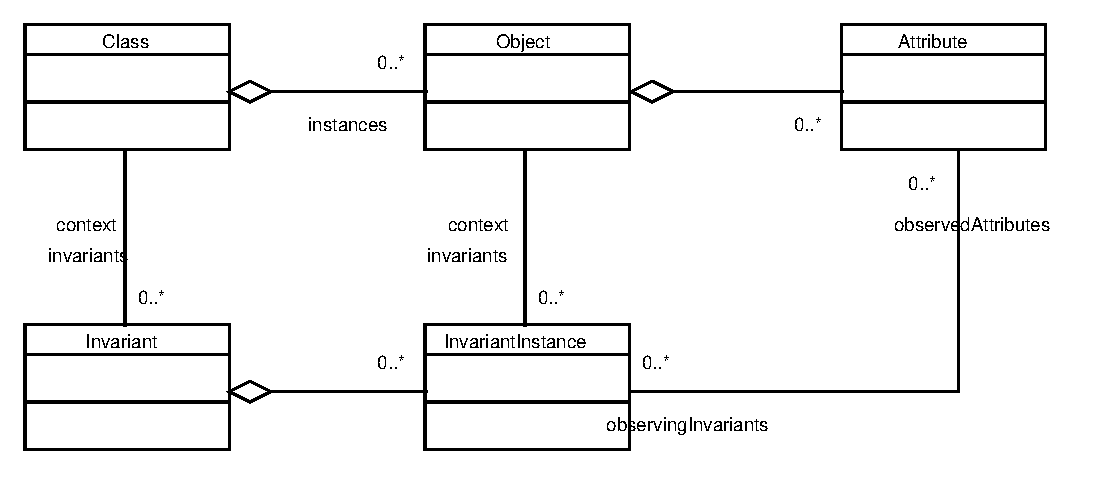
\includegraphics{observingInvariants.eps}} \par}


\caption{Design for Observing Invariants\label{Abb:observingInvariants}}
\end{figure} 

The classes in the UML chart have the following meaning:

\vspace{0.3cm}
{\centering \begin{tabular}{|l|l|l|}
\hline 
Class&
&
Example\\
\hline 
\hline 
Class&
An arbitrary class of &
\texttt{class~Person}\\
&
the user model&
\\
\hline 
Invariant&
An invariant in the &
\texttt{context~Person} \\
&
context of a class&
\texttt{inv:~age>=0}\\
\hline 
Object&
An instance of a class&
Person Joe\\
\hline 
Invariant-&
An invariant in the &
Has Joe \\
Instance&
context of an object.&
a positive age?\\
\hline 
Feature&
A feature (attribute or &
Joe's age\\
&
query method) of an object.&
\\
\hline 
\end{tabular}\par}
\vspace{0.3cm}

For now, lets think of features as attributes only. How to deal with query methods
is explained below. 

The cycle of checking invariants contains two stages.

\begin{enumerate}
\item Evaluating invariants. When evaluating an invariant instance, this invariant
instance registers to all object attributes used during evaluation as observer.
This means, the attribute promises to notify the invariant instance, when the
attributes value changes.
\item Running the model. When an attribute changed its value during execution of user
code, it notifies all observing invariant instances. Then, the attribute unregisters
all observers, so they must register again on the next evaluation stage. See
section \ref{Sec:structuralScopeImplementation} how changed attributes are
detected.
\end{enumerate}
This design can be extended to query\footnote{
Operations used in ocl expressions must not have side effects.
} methods. If the query does not have parameters, it's exactly like attributes.
Things get a bit more complex, if the queries are parameterized. See figure
\ref{Abb:observingMethods}.

\begin{figure}
{\centering \resizebox*{1\columnwidth}{!}{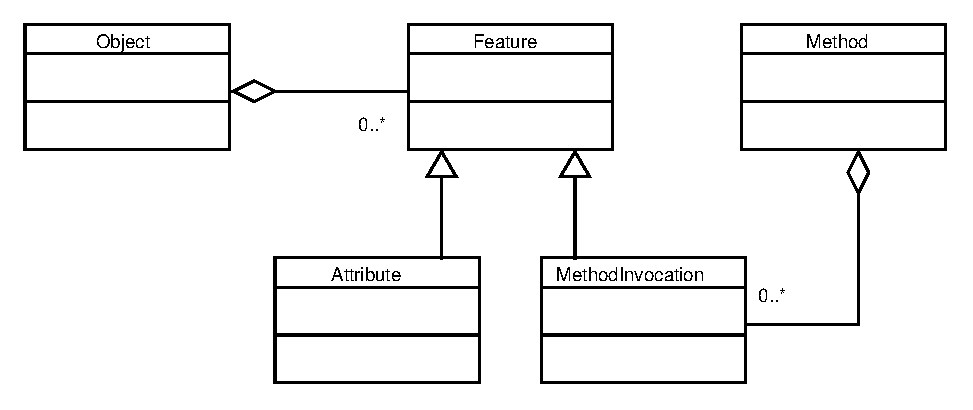
\includegraphics{observingMethods.eps}} \par}


\caption{Design for Observing Methods\label{Abb:observingMethods}}
\end{figure}

The point is, that not methods but method invocations are features observed
by invariants. A method invocation is a method together with a parameter sequence
suitable to invoke this method. 

Up to now, the implementation observes attributes only.


\subsection{Implementation\label{Sec:structuralScopeImplementation}}

Not all of these classes exist explicitly in the implementation. \emph{Class}
and \emph{Object} are provided by the user model already. \emph{Invariant} exists
only as an additional method \texttt{check\-Ocl\-Invariant\_\-<name>} of
its context class. \emph{InvariantInstance} is an explicit class\footnote{
called a bit confusingly \texttt{tudresden.ocl.injection.lib.Invariant}.
} of the instrumentation runtime library. Finally \emph{Feature} is provided
by the user model, but cannot be referred to as a single java object. (\texttt{java.\-lang.\-reflect.\-Field}
is a field of a class, not of an object.) Whenever a feature has to be referred
to, it is represented by it's observer collection object, which is sufficient
for the needs of this implementation.

Changes of object features are detected with polling. For each feature a backup
attribute is added to the class. 

\begin{lyxcode}
class~Person\\
\{\\
~~int~age;\\
~~int~age\_oclbackup=age;\\
\}
\end{lyxcode}
Additionally there is a utility method added comparing each attribute to it's
backup. If there is a difference, the observers of the attribute are notified. 

\begin{lyxcode}
private~void~checkForChangedFeatures()\\
\{\\
~~if(age!=age\_oclbackup)\\
~~\{\\
~~~~age\_oclbackup=age;\\
~~~~//~notify~observers~of~age\\
~~\}\\
~~//~...~further~attributes\\
\}

~
\end{lyxcode}
This method is called immediately before and after each method of the class.
If the attribute contains an object reference, the comparison tests object identity,
not object equality. This means, the \texttt{!=} operator is used as for basic
types and not the \texttt{equals()} method. 

For collections the backup stores a hashcode of the collection to avoid the
overhead of maintaining a complete backup collection. Since comparison to backups
is done very often, hashcode computation is required to be lightweight. The
following section discusses this in detail.


\subsection{Detecting Collection Modification\label{Sec:detectingCollectionChanges}}

Detecting changes of attributes is essential for caching of invariants as described
above. For atomic attributes this is trivial: \texttt{age!=age\_backup} does
it all. For collection attributes it's not that easy. The backup of a collection
shouldn't be a collection as well, since this would consume large amounts of
memory. Also, comparison between two collection isn't that fast.

Thus, the backup for collection attributes stores a single integer value only.
This value is computed from the collection. When the collection changes, also
the value is expected to change. Such a value is commonly referred to as hash
value. 

However, these hash values are not required to be uniformly distributed. Also,
the hash value is required to be constant for unmodified collections only, not
generally for equal collections. This means: if an element is added to the collection
and removed immediately afterwards, the collection is \emph{not} required to
have the same hash code as before. This relaxion of requirements will be used
below. It has to be admitted, that the term ``hash code'' is used here mainly
for historical reasons.

A first try to implement the hash functions follows the implementation of \texttt{hashCode}
methods in the Java Collection API. These methods cannot be used directly, since
they call method \texttt{hashCode} for each of their elements. This is not desired,
since change detection covers object identity, not object value. To achieve
the intended behavior, collection hash functions had to be rewritten with calls
to \texttt{System.identityHashCode}. This has been implemented in class \texttt{HashExact}\footnote{
All the source code is in \texttt{tudresden.injection.lib.Hash{*}.java}.
}.

These hash functions are good at detecting changes. However, they are too slow.
Each invocation involves an iteration over the whole collection. For object
populations of a few hundert instances with many relations between them, this
virtually causes the system to stop.

A quick but incomplete fix is achieved with the hash functions in \texttt{HashSize}.
They simply return the size of the collection. This is very quick of course.
But it does not detect changes which don't affect the collections size.

Finally, \texttt{HashModCount} performs a hash function which is a) nearly as
fast as \texttt{HashSize}, but b) performs change detection even better than
\texttt{HashExact}. It uses the fact, that standard collections already provide
a change detection mechanism for implementing fail-fast iterators. Each collection
maintains a modification counter, which is incremented whenever the collection
is modified. Iterators create a copy of this counter on creation, and check
this copy on every access. Unfortunately, the counter isn't publicly available.
Thus, \texttt{HashModCount} has to access the private counter attribute via
reflection. This is highly dependent on the internal details of collection classes.
The implementation has been tested successfully on JDK 1.2.2. With other versions
better do not expect it to work.

There is a work-around for this. The collection backup could be an iterator
instead of an integer. To detect a modification, just access the iterator and
wait for a \texttt{ConcurrentModificationException}. This has not been implemented
yet, since it imposes several problems. Method \texttt{hasNext()} does not check
for modifications. Thus, method \texttt{next()} has to be invoked. But this
may also fail due to \texttt{NoSuchElementException} if there are no elements
left. Thus, the iterator used for backup would have to be recreated, whenever
there is no element left. Empty collections would require a special treatment.

Using the fail-fast mechanism obviously does not work for arrays. However, a
fall back to \texttt{HashExact} or \texttt{HashSize} is easily provided. This
could even be decided dynamicely depending on the size of the arrays.

The table below summarizes the different detection mechanisms:

\vspace{0.3cm}
{\centering \begin{tabular}{|c|c|c|c|c|}
\hline 
&
Exact&
Size&
ModCount&
Iterator\\
\hline 
\hline 
Modification &
nearly perfect&
insertion/&
perfect&
perfect\\
Detection&
&
deletion only&
&
\\
\hline 
Runtime &
linear&
constant/&
constant/&
constant/\\
Complexity&
&
very low&
low&
intermediate\\
\hline 
Implemention&
yes&
yes&
yes&
-\\
\hline 
\hline 
Works with&
&
&
&
\\
\hline 
\hline 
Arrays&
yes&
yes&
fall back &
fall back\\
&
&
&
to other&
to other\\
\hline 
Collections without &
yes&
yes&
runtime&
silent\\
Fail-Fast Iterators&
&
&
error&
failure\\
\hline 
 Non-JDK &
yes&
yes&
runtime &
yes\\
Collections with &
&
&
error&
\\
Fail-Fast Iterators&
&
&
&
\\
\hline 
JDK Standard &
yes&
yes&
yes&
yes\\
Collections &
&
&
&
\\
\hline 
\end{tabular}\par}
\vspace{0.3cm}

Finally there is the question, which to choose. Probably one should start with
\emph{Exact} (the default). If this works, everything is fine. If the application
slows down more, than one is willing to accept, try \emph{ModCount} (invoked
with option \texttt{-{}-modcount-hash}). If this works, it's fine. Otherwise
it will fail-fast throwing a \texttt{RuntimeException}. Then one may try \emph{Size}
(\texttt{-{}-simple-hash}). Hopefully it doesn't miss too many modifications. 

If this is not acceptable, one may implement the \emph{Iterator} method. It
is important, that all collections used in the application provide fail-fast
iterators (JDK standard collections do). Otherwise modifications may be missed
silently.

\cleardoublepage


\chapter{Model Information \label{Sec:chapterModelInformation}}

The OCL compiler needs model information for type checking. How this works is
explained in \cite{ff3} section 5.3.3. 

One possible source of model information may be a UML model exported from a
CASE tool. This is probably the most elegant way. But since most real-world
projects don't have a (up to date) UML representation of their business model,
this isn't feasible in practice.

Another source is the java code itself, accessed through the reflection API\footnote{
see class \texttt{tudresden.ocl.check.types.ReflectionFacade}.
}. This is very convenient, since no additional model is needed. However, java
reflection lacks some model properties which are important for type checking.

\begin{enumerate}
\item Element types of collections, particularly collections representing associations.
From a C++ perspective, java lacks templates implementing parameterized container
classes.
\item Qualifier types of maps, representing qualified associations.
\item The isQuery tag of operations. Note, that OCL expressions may use operations
without side effects (queries) only.
\end{enumerate}
This chapter presents a solution to the first two items above. The information
needed is put into the source code. Section \ref{Sec:element_type_tag} explains,
how this information is stored, while section \ref{Sec:ReverseEngineering}
presents several approaches, how this information is generated.

The third item could be solved in a similar way, by putting an isQuery tag into
the source code. However, this is not an urgent problem. Without an explicit
solution the developer has to be careful to call java methods without side effects
only in OCL expressions.


\section{Representing Element Types\label{Sec:element_type_tag}}

Element types and qualifier types are specified using special tags in javadoc
comments. See the example below. 

\begin{lyxcode}
class~Company\\
\{\\
~~/{*}{*}\\
~~~~~All~persons~employed~by~this~company.\\
~~~~~@element-type~Person\\
~~{*}/\\
~~Collection~employees;\\
\}
\end{lyxcode}
The \texttt{@element-type} tag takes an parameter specifying a java class or
interface. Thus, it's similar to \texttt{@see} as defined in \cite{JAVA} section
18.4.1. The \texttt{@element-type} tag is valid for attributes only, and there
must be at most one such tag per javadoc comment. The tag is not restricted
to attributes of type \texttt{java.util.Collection}, since future implementations
could use other collection API's as well.

Analogously, the \texttt{@key-type} tag is introduced for association qualifiers. 

\begin{lyxcode}
class~Bank\\
\{\\
~~/{*}{*}\\
~~~~~Customers~qualified~by~their~account~number.\\
~~~~~@element-type~Person\\
~~~~~@key-type~Integer\\
~~{*}/\\
~~Map~customers;\\
\}
\end{lyxcode}
Note, that the reflection model is restricted to qualified associations with
one qualifier only. \cite{UML} allows multiple qualifiers, but there is no
convenient representation for this in java. 

Furthermore, UML specifies a qualified association which has not been qualified
in the OCL expression to be a set, i.e. there must be no duplicates. For the
java example above, this means, that the following invariant must hold:

\begin{lyxcode}
context~Bank~inv:~\\
~~customers->size()=customers->asSet()->size()
\end{lyxcode}
Since this is not enforced by \texttt{java.util.Map} (only keys are guaranteed
to be unique), the OCL library provides an appropriate runtime check.


\paragraph{Implementation.}

A really comfortable implementation would let the java compiler do the parsing,
and provide the information through an extended reflection API. This would be
similar to the \texttt{@deprecated} tag. However, this approach would require
the java compiler, the JVM and the standard runtime library to be modified.
Apart from the effort of making these modifications, most java developers probably
have a profound aversion against using a dedicated java environment just for
checking OCL constraints.

The implementation developed with this paper extends\footnote{
Encapsulated in \texttt{tudresden.ocl.check.types.ReflectionExtender}.
} the reflection facade by scanning the source code for these comments on demand.
This implies, that the java source code is necessary for type checking OCL constraints
in addition to the class files.

There is a crucial question left: Where do the tags come? Possible sources are:

\begin{itemize}
\item A UML model. The code generator of a CASE tool could generate these tags. 
\item Maintained by hand. It is good-practice of programming, to specify which kind
of objects are supposed to be in a collection attribute. The tags just make
this information available formally. 
\item Reverse Engineering. This is discussed in detail in section \ref{Sec:ReverseEngineering}
below.
\end{itemize}
Collection attributes with type tags are verified on runtime by the instrumented
code. Note, that this kind of type information is useful for reverse engineering
a UML model from given java code.


\section{Reverse Engineering\label{Sec:ReverseEngineering}}

Section \ref{Sec:element_type_tag} explained, how to store additional type
information of a java model in javadoc tags. This section discusses, how to
create this information.

Actually, these type tags have to be created manually. None of the automated
procedures is perfect, so these procedures are suitable for decision support
only. This chapter tries to support the developer with an interactive tool for
inserting \texttt{@element-type} and \texttt{@key-type} tags into the code.
There are two main features of this tool:

\begin{enumerate}
\item Graphical User Interface: Clear presentation of missing type tags and comfortable
editing facilities. 
\item Decision Support: Giving hints to the developer. These hints are either derived
statically (section \ref{Sec:ReverseEngineeringStatic} and \ref{sec: ReverseEngineeringWomble})
or gathered dynamically on runtime (section \ref{Sec:ReverseEngineeringDynamic}).
There should be a special indication, if several hints suggest different types.
\end{enumerate}
A prototype\footnote{
run class \texttt{tudresden.ocl.injection.reverseeng.RevengGUI}.
} of this tool according to the ideas presented in this section has been developed
by Steffen Zschaler. The prototype currently features the graphical user interface
and the runtime analysis of section \ref{Sec:ReverseEngineeringDynamic}.


\subsection{Source Code Analysis\label{Sec:ReverseEngineeringStatic}}

Information about element types may be derived from static properties of the
class, such as parameter types of methods and other tags in javadoc comments. 

The following example suggests some of these properties. The element type of
\texttt{employees} is obviously \texttt{Person}, but this information is not
yet available to the OCL compiler. The tool could derive an appropriate hint
for the developer from each of the underlined features.

\begin{lyxcode}
/{*}{*}\\
~~~All~employed~\{@link~\underbar{Person}~persons\}~of~this~company.\\
~~~@see~\underbar{Person}\\
{*}/\\
Collection~employees;\\
~\\
boolean~isEmployee(\underbar{Person});\\
void~addEmployee(\underbar{Person});\\
void~removeEmployee(\underbar{Person});
\end{lyxcode}
Note, that the example above requires linguistic knowledge about plural and
singular form of nouns (employee here). This gets far more difficult, if identifiers
are not English.


\subsection{Runtime Analysis\label{Sec:ReverseEngineeringDynamic}}

This section describes, how to trace element types of collections on runtime.
This is useful, if there is no static type information available, as described
in the previous section. 

For each collection attribute, the object types encountered during a run of
the program are collected and fed into the interactive tool. This requires the
program to be executable. Additionally there must be extensive test cases available,
otherwise only a subset of all possible element types will be encountered.

The interactive tool presents the set of object types for every collection attribute.
Additionally, the tool highlights all types, for which there is no super type
in this set. Formally, these are the local minima of the set respective to the
generalization partial order. These local minima are good candidates for an
element type, especially if there is only one minimum. Presenting minima simplifies
the decision if there are many types encountered in the collection attribute.


\paragraph{Implementation.}

The instrumented code makes a static method \texttt{traceTypes}\footnote{
Actually \texttt{tudresden.ocl.injection.lib.TypeTracer.traceTypes}.
} to be executed whenever a collection attribute changes its contents. Class
\texttt{TypeTracer} maintains a static data structure containing all element
types and key types for all attributes, as well as the minima of these type
sets. This information is continuesly written to a log file. The interactive
tool can read this log file and display the information.


\subsection{Byte Code Analysis \label{sec: ReverseEngineeringWomble}}

This section describes how type information can be extracted from java byte
code. This technology and its implementation (called Superwomble) was developed
by Daniel Jackson and Allison Waingold at the MIT. This section outlines the
parts of their paper (\cite{womble}) related to type information together with
experiences from practical experiments with the tool.

Superwomble is a powerful reverse engineering solution. It generates object
graphs from nothing but java byte code. Object graphs are roughly speaking a
subset of UML class diagrams. They feature classes with generalizationships
and associations between them. The graph is finally fed into a tool named dot,
which does a nice layout for the graph.

One of the tricky parts of this tool is the detection of element types for object
containers, which is exactly what this whole chapter is about. How this works,
is explained on the Company-Person example from section \ref{Sec:element_type_tag}
(page \pageref{Sec:element_type_tag}). 

Suppose \texttt{company} is a variable of type \texttt{Company} and \texttt{person}
of type \texttt{Person}. A typical program around this example would probably
contain a statement like this:

\begin{lyxcode}
company.employees.add(person);
\end{lyxcode}
The operation \texttt{add} takes an argument of type \texttt{Object}, but is
called with a variable of type \texttt{Person}. This is a good hint, that the
element type of \texttt{employees} is \texttt{Person}.

The same works for objects returned from the container. The expression

\begin{lyxcode}
person=(Person)(company.employees.iterator().next());
\end{lyxcode}
strongly suggests the element type \texttt{Person}.

Another highlight of Superwomble is, that container classes are detected even
if they don't implement \texttt{java.util.Collection}. In fact the type is not
cared at all. Instead there are some heuristics applied to decide, whether a
class is an object container or not.

The tool was used on several parts of both the OCL toolkit and the net-linx
code, and it produced good and reliable results.

Integration of Superwomble results into the interactive tool should be possible.
The object graph is exported to a human readable text file. However, this task
is outside the scope of this paper.


\subsection{Comparison}

This section provides a comparison between the three approaches presented in
the sections above. 

\vspace{0.3cm}
{\centering \begin{tabular}{|l||c|c|c|}
\hline 
&
Source Code&
Byte Code&
Runtime\\
&
&
(Superwomble)&
\\
\hline 
\hline 
Source Code required&
yes&
no&
yes\\
\hline 
Required Code Quality&
fairly &
fully &
up and \\
&
parseable&
compileable&
running\\
\hline 
Availability of Results&
intermediate&
good &
good\\
\hline 
Reliability of Results&
good&
very good&
intermediate\\
\hline 
Application Effort&
low&
low&
high\\
\hline 
Implementation Effort &
low&
high&
very low\\
(starkly subjective)&
&
&
\\
\hline 
Availability&
LGPL&
Binary at no cost&
LGPL\\
\hline 
\end{tabular}\par}
\vspace{0.3cm}

Runtime analysis requires the source code to be instrumented before. Only byte
code analysis requires no source code. This argument is weakened by the fact,
that the type information is to be inserted into source code anyway. However,
byte code analysis may cover libraries, which aren't available in source code,
but provide useful type information about other parts of the program.

Anyway, byte code analysis requires, that there is a fully compilable source
code somewhere, even if it's not available to the user. Source code analysis
even makes do with incorrect source code, as long as signature data is parsable
(method headers etc.) and method bodies hold the bracket balance. Most demanding
on source code quality is runtime analysis, which requires a running system,
with complete test cases.

Source code analysis is most demanding on the ``beauty'' of implementation.
To deliver results, it requires some kind of getter/setter methods for the container
attributes. In contrary, byte code and runtime analysis even work for public
container attributes manipulated from outside of the class.

For runtime analysis \emph{reliability of results} depends heavily on completeness
of test cases. If the test cases are insufficient, results may be wrong. Byte
code analysis provides best reliability, it's more difficult for a poor quality
code to fool the analysis.

Runtime analysis also requires most \emph{application effort} for the user.
The system must be actually run. Particularilly all requirements for runtime
(libraries, database, configuration etc.) must be available.

The \emph{implementation effort} is very subjective for this paper. Both source
code and runtime analysis require parsing and instrumenting of java source code,
which was already built for runtime verification of OCL constraints. Thus the
implementation effort in this paper was low. Byte code analysis is something
completely different.

Finally, \emph{availability} is about whether it is allowed to use, review and
adapt the implementation. According to \cite{freesw}, the difference between
\emph{LGPL} and \emph{Binary at no cost} is same as between free speech and
free beer.


\subsection{Summary}

There have been three approaches presented for acquiring type information. Runtime
analysis is implemented and fully integrated into the project. Source code analysis
is not yet implemented, but this should be easy to add. Experiences with byte
code analysis where drawn from the tool Superwomble (\cite{womble}). This is
fully implemented but not integrated into the OCL toolkit, thus not ready to
use.

Adding up the scores, byte code analysis is probably the best. However, most
of the criteria listed above are some kind of orthogonal, so adding up scores
might not be sufficient for a decision. Each application may emphasize different
criteria, so a universal solution is not available.

All approaches have one thing in common: they are not perfect. Thus, they cannot
be used directly in the type checker of the OCL compiler. The intermediate step
of the \texttt{@element-type} tags is necessary to allow correcting intervention
of a human user.

\cleardoublepage


\chapter{Industrial Example \label{Sec:chapterIndustrial}}

For practical experiments with an industrial strength project, the partner net-linx
AG provided the source code of its emerging product nxCom. 

The product is a three tier solution providing a business directory service.
There is a core business logic module, a maintance interface implemented with
Java Swing and a customer web interface using Java Server Pages.

The experiments where limited to the business logic module. It consists of 245
classes and 17131 lines of code. Persistence is realized using the Versant ODBMS
and the Java Versant Interface (JVI) \cite{Versant}. The OCL toolkit does not
work together with JVI due to a bug in the latter. (This bug has been fixed
after submission of this paper.) A detailed analysis can be found in appendix
\ref{sec: VersantProblem}. For the test a special developer configuration was
used, which employs a XML file for realizing persistence.

For experimentation 10 invariants have been developed and inserted into this
module. It wouldn't make much sense to give an introduction into the business
logic module, therefore the actual constraints have been transformed into analogous
counterparts for the Person - Company model used in \cite{Warmer}:

\begin{itemize}
\item 5 invariants checking the consistency of bidirectional associations such as:
\end{itemize}
\begin{lyxcode}
context~Person~inv~employers\_back:~

~~employers->forAll(employees->includes(self))~
\end{lyxcode}
\begin{itemize}
\item 3 invariants where several attributes where tested for consistency to the object's
current state in life cycle, such as:
\end{itemize}
\begin{lyxcode}
context~Person~inv:

~~isMarried~implies~(wife->isEmpty~xor~husband->isEmpty)
\end{lyxcode}
\begin{itemize}
\item one invariant ensuring a minimum cardinality of an association:
\end{itemize}
\begin{lyxcode}
context~Company~inv~has\_employees:~

~~employees->size>0
\end{lyxcode}
\begin{itemize}
\item and finally one invariant checking the consistency of a redundant attribute,
in this case the uppercase version of a string:
\end{itemize}
\begin{lyxcode}
context~Company~inv:~

~~uppername=name.toUpper
\end{lyxcode}
The impact of code instrumentation on the size of the module is shown in the
table below. Lines of Code where determined using CCCC \cite{cccc}). Execution
times where measured on a AMD Athlon 600 system.

\vspace{0.3cm}
{\centering \begin{tabular}{|c||c|c|}
\hline 
&
Original Code&
Instrumented Code\\
\hline 
\hline 
Size of Source Code&
 1.1 MB&
3.2 MB\\
\hline 
Lines of Code&
 17131 &
43587 \\
\hline 
 (Re-)Instrumentation &
36 s&
91 s\\
\hline 
(Re-)Cleaning &
23 s&
73 s\\
\hline 
\end{tabular}\par}
\vspace{0.3cm}

Running the instrumented code revealed a number of constraint violations. Some
of them have been reconstructed by hand, and turned out to be inconsistencies
in the test data. Due to the amount it was not possible to correct these inconsistencies
within this work.

\cleardoublepage


\chapter{Summary \label{Sec:chapterSummary}}

In this work, a java source code instrumentation tool has been developed. This
tool allows to insert code generated by the OCL compiler into arbitrary user
code. The instrumentation features an insertion scheme called method wrappers,
which seems to be new in respect to the related work researched by the author.
The insertion scheme provides a reversible instrumentation. This means, that
the instrumented code can be modified without losing all changes on the next
instrumentation. 

A concept for caching results of invariants has been developed and partially
implemented. 

The OCL type checker was extended to gather additional information from javadoc
tags. This makes the OCL compiler fully independent of a UML representation
of the java code. A concept for generating such tags and inserting them into
the java code has been developed. This concept has been partially implemented
by Steffen Zschaler. 

The existing OCL compiler has been maintained and slightly extended. These extentions
provide additional flexibility needed for the components developed in this work.
Coupling beetween existing and new components is kept low by restricting dependencies
to java interfaces.

The tool has been experimented with using the java source code of an industrial
application. For this application, a small set of typical constraints has been
developed.

The OCL tool is still far from being complete. Some ideas for future work are
discussed in the next chapter. However, the tool seems to be in a condition,
where an early adopter could actually start using it for some real world task. 

\cleardoublepage


\chapter{Outlook \label{Sec:chapterOutlook}}

The results of this paper leave various directions for future work on the OCL
toolkit. This chapter outlines the (in the author's opinion) most interesting
ideas.


\section{Inheriting Constraints}

Inheriting constraints is completely neglected in the current version. This
means, that a subclass does not inherit the constraints of its ancestors. At
a glance this is an implementation problem only. But it is not that easy.

Simply promoting constraints of a class to all its descendants is not sufficient.
This downward promotion implies a conjunction (logical AND) of inherited and
own constraints. This is suitable for invariants and postconditions, but not
for preconditions. Design by Contract (DbC) requires inheritance of \emph{contracts},
not just constraints, thus preconditions cannot be strengthened. To make this
sure, DbC suggests a disjunction (logical OR) of inherited and own preconditions.

This causes some uncomfortable effects. Consider a class representing a bank
account. The account has an attribute \texttt{balance} and a method for drawing
money. There is no debit allowed, and for some technical reason the amount to
be drawn cannot exceed 10000 per transaction. This could be expressed like this:
(Postconditions have been omitted for brevity).

\begin{lyxcode}
context~Account::drawMoney(amount:integer)

~~pre:~amount<=10000

~~pre:~balance-amount>=0
\end{lyxcode}
A subclass weakens the second precondition by allowing a debit of 1000. 

\begin{lyxcode}
context~DebitableAccount::drawMoney(amount:integer)

~~pre:~balance-amount>=(-1000)
\end{lyxcode}
But what happened now? The effective precondition of DebitableAccount (\emph{ORing}
preconditions of both classes) is now just balance-amount>=(-1000). The upper
limit for amount disappeared. This is perfectly compatible with DbC, but certainly
not the intention of the developer.

A work-around is to repeat the upper limit for amount in the subclass. But this
is not convenient, particularly when considering 10 such technical preconditions
instead of just one. 

A sensible solution should allow to inherit a precondition as such without repeating
it in the subclass. A suitable solution could feature named preconditions and
a ``per name'' disjunction of these:

\begin{lyxcode}
context~Account::drawMoney(amount:integer)

~~pre~max\_amount:~~amount<=10000

~~pre~min\_balance:~balance-amount>=0

~

context~DebitableAccount::drawMoney(amount:integer)

~~pre~min\_balance:~balance-amount>=(-1000)
\end{lyxcode}
These considerations suggest, that there is still some investigation and development
needed to make the OCL toolkit usable for supporting Design by Contract.


\section{Integration with CASE Tools}


\subsection{Code Generation}

The OCL toolkit works with arbitrary java source code. Thus, it is definitely
compatible with java code generators of all CASE tools. Still, there are some
issues to be mentioned.


\paragraph{Export of OCL. }

If the CASE tool is able to store OCL constraints, there should be some export
function for them as well. A sophisticated export function could even embed
the constraints into javadoc comments (section \ref{Sec:embedConstraints}),
providing a single source solution. This should be easy to implement for CASE
tools with the source code available, otherwise the feasibility depends on API's
of the CASE tool.


\paragraph{Export of Element Types.}

Even more important is the export of \texttt{@element-type} javadoc tags (section
\ref{Sec:element_type_tag}). These are needed for type checking of constraints.
The feasibility of such an extension depends again on the availability of either
the source code or suitable API's.


\paragraph{Superseding Name Adapters.}

Code generators of Argo/UML \cite{Argo}, Rational Rose \cite{Rose} and Together
\cite{Together} require the employment of name adapters. This is, since an
association end called \texttt{employers} does not result in a collection attribute
of the same name, as one would expect. Instead, the attribute is called \texttt{myEmployers},
\texttt{theEmployers} or \texttt{lnkEmployers}, depending on the CASE tool.
The necessary translation is encapsulated in name adapters. It would be nice
to make code generators use the original name. This would remove the need for
name adapters, making the OCL toolkit and its application a bit less complex.


\subsection{Reverse Engineering }

The OCL toolkit provides support for inserting and validating \texttt{@element-type}
javadoc tags into arbitrary source code. This information could be used for
reverse engineering from Java to UML.

This significantly changes the way of reverse engineering: Up to now, a CASE
tool analyses the source code, and wherever there is some information missing
(particularly the element type of container attributes) it makes some simple
assumptions. In a second step, the user is expected to review the results and
adjust them where necessary.

The OCL toolkit can be used to swap the order of steps. First, the missing information
is inserted into the source code in form of \texttt{@element-type} tags. This
information is then used by the CASE tool to straightly produce a correct UML
model. The advantage is, that the additional information can be verified using
the runtime checks provided by the OCL toolkit.

Of course, the \texttt{@element-type} tag does not provide all the needed information.
For instance bidirectional associations cannot be determined, since they cannot
be distinguished from two independent one-way associations. This could be approached
by introducing some kind of \texttt{@reverse-direction} tag. Given the infrastructure
already provided, such extensions should be easy to implement.

These considerations suggest, that the OCL toolkit together with a CASE tool
could be extended into a complete round trip engineering solution - with special
support for starting the round trip at the ``java side'' of the circle.


\section{Others}


\paragraph{Reduce Observed Attributes.}

Caching of invariants (section \ref{Sec:structuralScope}) requires observing
object attributes for modifications. Up to now, all attributes found in the
java source code are observed, regardless whether they are used in some OCL
expression or not. This could be reduced to those attributes, which are actually
referred to in any of the constraints. This would significantly improve runtime
efficiency of the instrumented code. For an implementation one would probably
intercept the OCL type checker to get the necessary information.


\paragraph{Observing Queries.}

Caching the results of invariants requires observing of both attributes and
query methods. However, observing queries has not been implemented yet. The
total approach to caching requires a significant memory overhead. Observing
queries will make this even worse by introducing another step of indirection.
This should not be attempted until this approach has shown to be functional
for big projects with many and complex invariants.


\paragraph{Java Constraints.}

Constraints could be expressed in Java instead of OCL. This may be useful for
developers, who are unfamiliar with UML and OCL. An advantage is, that such
a tool would be dramatically smaller and faster. A serious drawback is the loss
of some quite comfortable functionality of OCL, such as universal and existential
quantifiers and \texttt{@pre} modifiers. Furthermore, caching of invariants
for java constraints requires much more implementation effort.


\paragraph{Enhancing Flexibility.}

Simply put, this means more options and probably some kind of configuration
file. A good example is iContract \cite{iContract}, which allows to enable
constraints independently for packages, classes and methods using a configuration
file. Additionally there could be a more flexible scope of invariants, as suggested
in section \ref{Sec:structuralScope}.

\appendix
\cleardoublepage


\chapter{Maintance of the OCL~Compiler \label{Sec:chapterMaintance}}

This chapter describes all major changes to Frank Fingers OCL compiler. This
includes bugfixes too, if they caused changes of internal or external interfaces.
It it some kind of update for \cite{ff3}, listing everything changed since.


\section{Reflection Facade and OCL Library}

Many changes occurred both in the reflection model facade and in the OCL library.
This section groups these changes.


\subsection{Polymorphism of Operation Parameters}

Both \texttt{Reflection\-Facade.\-navigate\-Parameterized} and \texttt{OclAny\-Impl.\-get\-Feature}
lacked polymorphism of operation parameters. This means, that a method is found
only if actual parameter types match formal parameter types exactly. The correct
behavior is, that actual parameter types may also be subtypes of formal parameter
types. For a detailed description see \cite{rw7} section 3.1.5. 

The new implementation made \texttt{Reflection\-Adapter.\-get\-Class\-ForType}
superfluous, so it was removed from the interface.


\subsection{Mandatory Name Adapters}

Previous versions of the OCL library provided a default functionality, if no
name adapter had been set explicitly.

Now it is mandatory to set a name adapter. Otherwise a NullPointerException
is thrown. The default functionality has been moved into a separate name adapter
(\texttt{Simple\-Name\-Adapter}) which is used in the reflection facade as
well. The name adapter may also be set by the java property \texttt{tudresden.\-ocl.\-lib.\-name\-adapter}.

\texttt{Argo\-Name\-Adapter} has been generalized into \texttt{Prefix\-Name\-Adapter},
which takes an arbitrary name prefix (``\texttt{my}'' for Argo/UML) as a constructor
parameter. Using this adapter with ``\texttt{lnk}'' and ``\texttt{the}''
should work for Together/J and Rational Rose.


\subsection{Qualified Associations}

The OCL support was enhanced by adding a simplified form of qualified associations
to the reflection facade and the OCL library. ``Simplified'' means, that there
may be only one qualifier attribute. 

Qualified associations are represented in java with \texttt{java.\-util.Map}
by default, but this may be changed by implementing \texttt{Reflection\-Adapter.\-isMap(Class)}.


\subsection{Type Mapping from OCL to Java.}

The mapping between OCL types and java types now supports the collections API
introduced in JDK version 1.2. The changes concern \texttt{Default\-Ocl\-Factory.\-getOcl\-Representation\-For(Object)}
and \texttt{Default\-Reflection\-Adapter.\-get\-Class\-ForType}. 

A special handling of \texttt{java.\-util.\-Vector} supports code generated
by Argo/\texttt{\-}UML. The static configuration variable \texttt{Ocl.\-TAKE\_\-VECTORS\_\-AS\_SET}
causes vectors to be mapped to sets, instead of sequences.

The new mapping is listed below.

\vspace{0.3cm}
{\centering \begin{tabular}{|c|c|c|}
\hline 
Java (java.util)&
take vectors as set&
OCL\\
\hline 
\hline 
List&
-&
Sequence\\
\hline 
Vector&
false&
Sequence\\
&
true&
Set\\
\hline 
Set&
-&
Set\\
\hline 
Map&
-&
Set (qualified)\\
\hline 
\end{tabular}\par}
\vspace{0.3cm}

Furthermore, arrays are now supported. They are mapped into sequences of the
appropriate element type.


\section{OCL Library}

Some modifications occurred in the OCL library only.


\subsection{Undefined Values}

Previous versions of the OCL library implemented undefined values as singletons
for each type. 

This was given up. Now undefined values carry the reason for their creation
with them. When the undefined value is tried to be evaluated, this reason is
added to the exception message. 

This made \texttt{Ocl.STRICT\_\-CHECKING} superfluous, so it was removed. Wherever
this property was used, the library now produces an undefined value, parameterized
with the message of the exception formerly thrown.

Undefined values were introduced at some other operations of OCL objects:

\begin{enumerate}
\item Method \texttt{OclCollection.\-set\-To\-Range} now creates an undefined collection
(instead of throwing an exception), if lower bound is greater than upper bound.
\item The methods \texttt{Ocl.to<OclType>(OclRoot)} now return an undefined value
of the appropriate type, if argument is undefined. 
\end{enumerate}

\subsection{Java Null Values}

Previous versions handled a special null value for OCL strings. This null value
behaved like an empty string for most cases (e.g. concatenation). However a
null string and an empty string were not equal. This was removed. Now a null
string does exactly behave like an empty string. 

Previous versions returned an undefined OCL collection, if the java collection
field was null. Now, null collections are treated exactly like empty collections.

This behavior is encapsulated into a new method \texttt{getOcl\-Representation\-For\-Null(Class)}
in \texttt{OclFactory}. This method is called in \texttt{OclAny\-Impl.\-get\-Feature}.


\section{Type Checker}

Previous versions of the type checker missed support for classifier \texttt{OclAny}
in class \texttt{Default\-Type\-Factory}. 

Method \texttt{getClassifier} in class \texttt{Type\-Factory} has been removed
and replaced by \texttt{Type\-Factory.get}.


\section{Java Code Generator \label{Sec:maintainJavaCodeGenerator}}


\subsection{Code Fragments for @pre}

Meaning of code fragments created for @pre expressions (TRANSFER, PREPARATION,
POST) has been changed. The new behavior is easier and more flexible for different
code instrumentation tools. For a description of the new behavior see section
\ref{Sec:codegeneration_result}. 

For the old behavior compare to \cite{ff3} section 7.1.2. Below, there is a
detailed comparison on the example used there.

The OCL expression is

\begin{lyxcode}
context~Person::getIncomeAfterTax(tax:Real):Real~post:\\
~~age~=~age@pre
\end{lyxcode}
The TRANSFER fragment generated is still the same:

\begin{lyxcode}
OclInteger~tudOclNode2;
\end{lyxcode}
However, the PREPARATION fragment has changed. Below, there is the old version.
The new version just lacks the parts set in italics.

\begin{lyxcode}
final~OclAnyImpl~tudOclNode0=Ocl.toOclAnyImpl(Ocl.getFor(this));

final~OclReal~tudOclOpPar0=Ocl.toOclReal(Ocl.getFor(tax));

final~OclReal~tudOclResult0=OclReal.UNDEFINED;

final~OclInteger~tudOclNode1=Ocl.toOclInteger(

~~~~tudOclNode0.getFeature(\char`\"{}age\char`\"{}));

\textit{final~OclInteger}~tudOclNode2=Ocl.toOclInteger(

~~~~tudOclNode0.getFeature(\char`\"{}age\char`\"{}));

final~OclBoolean~tudOclNode3=tudOclNode1.isEqualTo(tudOclNode2);

\textit{this.tudOclNode2=tudOclNode2;}
\end{lyxcode}
The POST fragment changed as well. Again, this is the old version, with the
new version lacking the first line put in italics.

\begin{lyxcode}
\textit{final~OclInteger~tudOclNode2=this.tudOclNode2;}

final~OclAnyImpl~tudOclNode0=Ocl.toOclAnyImpl(Ocl.getFor(this));

final~OclReal~tudOclOpPar0=Ocl.toOclReal(Ocl.getFor(tax));

final~OclReal~tudOclResult0=Ocl.toOclReal(Ocl.getFor(result));

final~OclInteger~tudOclNode1=Ocl.toOclInteger(

~~~~tudOclNode0.getFeature(\char`\"{}age\char`\"{}));

final~OclBoolean~tudOclNode3=tudOclNode1.isEqualTo(tudOclNode2);
\end{lyxcode}
The old code fragments were intended to be inserted into the user code as follows:

\begin{lyxcode}
public~class~Person~

\{

~~//~TRANSFER~FRAGMENT

~

~~public~double~getIncomeAfterTax(double~tax)~

~~\{

~~~~getIncomeAfterTaxPRE(tax);

~~~~//~USER~CODE

~~~~getIncomeAfterTaxPOST(tax,~result);

~~~~return~result;

~~\}

~

~~private~void~getIncomeAfterTaxPRE(double~tax)

~~\{

~~~~//~PREPARATION~FRAGMENT

~~\}

~

~~private~void~getIncomeAfterTaxPOST(double~tax,~double~result)

~~\{

~~~~//~POST~FRAGMENT

~~\}

\}
\end{lyxcode}
With the new fragments, this still works. However, it's also possible to insert
the TRANSFER fragment into the method, thus making it a local variable:

\begin{lyxcode}
public~class~Person~

\{

~

~~public~double~getIncomeAfterTax(double~tax)~

~~\{

~~~~//~TRANSFER~FRAGEMENT

~~~~\{

~~~~~~//~PREPARATION~FRAGMENT

~~~~\}

~~~~//~USER~CODE

~~~~\{

~~~~~~//~POST~FRAGEMENT

~~~~\}

~~~~return~result;

~~\}

\}
\end{lyxcode}
The code instrumentation developed with this paper uses the second insertion
scheme only.


\subsection{Explicit Package Qualifiers.}

The java code generator now optionally prepends the explicit package qualifier
\texttt{tudresden.ocl.lib.} to OCL library classes. This makes an import statement
superfluous, and therefore fulfills the corresponding requirement in section
\ref{Sec:injection_requirements_reversable}.

\cleardoublepage


\chapter{Usage of the OCL Tool \label{Sec:chapterUsage}}

This chapter describes, how to use the instrumentation tool. Section \ref{Sec:UsageExample}
contains an example quickly demonstrating the main features. Section \ref{Sec:UsageReference}
provides a complete reference of the command line options.


\section{Example\label{Sec:UsageExample}}


\paragraph{Step 1:}

First, get the following files: dresden-ocl-injector.jar, xerces.jar and royloy.jar.
These files are available on our website at dresden-ocl.sourceforge.net or may
be produced from the sources using the \texttt{makeJar} script. Put these files
into one directory and change into that directory.

The file royloy.jar contains the example code. To unzip it type:

\begin{lyxcode}
jar~-xf~royloy.jar
\end{lyxcode}
You may now have a look at the example code, its in tudresden/ocl/test/royloy/.
The java code already contains OCL expressions in javadoc comments, for an easy
start see \texttt{Person.java} and \texttt{Company.java}. Additional OCL is
in the file \texttt{oclexpressions}.


\paragraph{Step 2:}

Now it's time to start the OCL tool. Type the following command on a single
line. Note, that the wildcards require a Unix shell to be expanded.

\begin{lyxcode}
java~-jar~dresden-ocl-injector.jar~\\
~~~-r~tudresden.ocl.test.royloy~\\
~~~-{}-modify~tudresden/ocl/test/royloy/{*}.java~
\end{lyxcode}
The example java code has now been modified. The modified code will have the
same behavior as the original code, but will additionally check the OCL constraints
embedded in the javadoc comments.


\paragraph{Step 3:}

To check this, compile the modified java code (again type everything on a single
line):

\begin{lyxcode}
javac~\\
~~~-classpath~dresden-ocl-injector.jar~\\
~~~tudresden/ocl/test/royloy/{*}.java
\end{lyxcode}
and 


\paragraph{Step 4:}

Run the test main function provided:

\begin{lyxcode}
java~\\
~~~-cp~.:dresden-ocl-injector.jar~\\
~~~tudresden.ocl.test.TestInjectionRoyloy~
\end{lyxcode}
Enjoy the messages about violated OCL constraints running down the screen. Messages
contain information about the violated constraint and the object involved.


\paragraph{Step 5:}

Clean the code from the modifications the OCL tool made.

\begin{lyxcode}
java~-jar~dresden-ocl-injector.jar~\\
~~~-{}-clean~-{}-modify~tudresden/ocl/test/royloy/{*}.java~
\end{lyxcode}
The example code is now exactly the same as you downloaded it.

Note, that the code actually was cleaned. No backups involved. To check this,
try the following:

\begin{enumerate}
\item Make a backup of one or more java files just before running the OCL tool (step~2).
\item After running the tool make some small modifications to the files, you made
a backup for. For example just add a single System.out.println to a method body.
\item Proceed until step~5.
\item Compare the cleaned code to your backup. 
\end{enumerate}
The difference will be just the small modifications you made.


\section{Reference\label{Sec:UsageReference}}

Synopsis is below.

\begin{lyxcode}
java~tudresden.ocl.injection.Main~{[}options{]}~file.java~..
\end{lyxcode}
Provide all java files to be modified. 

Options recognized are below. Most options have a short and a long version.
Long versions try to be self explanatory and should be used in scripts.

\begin{lyxcode}
-m~-{}-modify
\end{lyxcode}
\begin{quotation}
Enables modifying java files. If not provided, the modified java code is written
to \texttt{file.java.injected}. This switch serves as a safety check, whether
you \emph{really} want to replace your source code with the output of the OCL
tool.
\end{quotation}
\begin{lyxcode}
-c~-{}-clean
\end{lyxcode}
\begin{quotation}
Performs cleaning of source files instead of instrumentation. After cleaning,
the source code should show no differences to the version before running the
OCL tool.
\end{quotation}
\begin{lyxcode}
-f~-{}-constraint-file~constraints.txt
\end{lyxcode}
\begin{quotation}
Specifies the text file containing the constraints. Usually not needed, since
constraints may and should be placed into javadoc comments. See section \ref{Sec:embedConstraints}.
\end{quotation}
\begin{lyxcode}
-r~-{}-reflection-model~modelpackage
\end{lyxcode}
\begin{quotation}
Specifies the java packages containing the model covered. If there is a constraint
\texttt{context~Person}, the type checker will look for class Person in all
packages given by this option. This is some kind of ``\texttt{import} for OCL''.
For multiple packages use multiple options.
\end{quotation}
\begin{lyxcode}
-n~-{}-name-adapter~{[}none|argo{]}
\end{lyxcode}
\begin{quotation}
Specifies the name adapter. Default is \texttt{none}. If you don't use code
generated by Argo/UML, the default is sufficient. Further information on name
adapters is available at \cite{ff3} section 3.5.1 and 3.5.6.
\end{quotation}
\begin{lyxcode}
-is~-{}-invariant-scope~

~~~~~~{[}all|private|protected|package|public|explicit{]}
\end{lyxcode}
\begin{quotation}
Specifies the the scope of invariants used. See section \ref{Sec:temporalScope}
for a detailed explanation. Access modifiers select methods having the same
or a more public access modifier. Thus, \texttt{all} and \texttt{private} are
equivalent. Default is \texttt{all}.
\end{quotation}
\begin{lyxcode}
-vm~-{}-violation-macro~macro
\end{lyxcode}
\begin{quotation}
Specifies what to do, if a constraint fails. This string is inserted verbatim
into the code. The OCL tool appends a pair of parents enclosing a suitable message
string. Good candidates are \texttt{System.\-out.\-println} (the default)
or \texttt{throw~new~RuntimeException}. Note, that the latter must be enclosed
in \texttt{\char`\"{}\char`\"{}} on Unix shells.

The exception thrown must not be a \emph{checked exception} as specified by
\cite{JAVA} section 11.2. Otherwise the modified code will not compile!
\end{quotation}
\begin{lyxcode}
-tt~-{}-trace-types
\end{lyxcode}
\begin{quotation}
Performs type tracing of collection elements. See section \ref{Sec:ReverseEngineeringDynamic}
for details. The information gathered is written to a log file specified by
property \texttt{tudresden.\-ocl.\-injection.\-lib.\-TypeTracer.log}.

Note, that the log file must be specified when running the user program, not
the OCL tool! For example use \texttt{-Dtudresden.\-ocl.\-injection.\-lib.TypeTracer.\-log=example.\-ocl\-type\-trace}.
If not specified, the type information is written to standard out.
\end{quotation}
\begin{lyxcode}
-{}-insert-immediately
\end{lyxcode}
\begin{quotation}
Triggers immediate insertion of wrapper methods. Otherwise wrapper methods are
inserted at the end of each class. Immediate insertion allows easier tracing
of the modifications. This option is mainly useful for debugging.
\end{quotation}
\begin{lyxcode}
-{}-trace-checking
\end{lyxcode}
\begin{quotation}
Adds code logging each constraint checked on an object to standard out. Useful
for debugging.
\end{quotation}
\begin{lyxcode}
-{}-simple-hash
\end{lyxcode}
\begin{quotation}
Uses simple hash functions in \texttt{HashSize}, instead of the sophisticated
hash functions in \texttt{HashExact}. Simple hash functions just return the
size of the collection, so they will detect insertions/deletions only. Reduces
CPU load for big models.
\end{quotation}
\begin{lyxcode}
-{}-modcount-hash
\end{lyxcode}
\begin{quotation}
Uses hash functions in \texttt{HashModCount}, instead of the hash functions
in \texttt{HashExact}. \texttt{HashModCount} functions are even better in modification
detection than functions in \texttt{HashExact}. Also, they are almost as fast
as \texttt{HashSize}. However, they heavily depend on internals of the java
collections implementation. Use at your own risk. See section \ref{Sec:detectingCollectionChanges}.
\end{quotation}
\cleardoublepage


\chapter{Code Examples \label{Sec:chapterCodeExamples}}


\section{Unreachable Post Condition Code in iContract\label{sec: unreachableIConstract}}

This appendix shows, that iContract cannot handle methods with an unreachable
end of method body as stated in section \ref{sec: compareIContract}.

The example is derived from the example code that accompanies iContract. The
following method provides such a situation: The \texttt{throw} statement in
the last line prevents the execution path from ever reaching the end of the
method body.

\begin{lyxcode}
/{*}{*}\\
~{*}~@post~age~>~0\\
~{*}/\\
public~void~setAge(~int~age~)\\
\{~\\
~~age\_~=~age;\\
~~throw~new~RuntimeException();\\
\}
\end{lyxcode}
Now the post condition has to be included into iContracts configuration, so
that it actually gets checked.

\begin{lyxcode}
iContract.doc.tutorial.Person.Employee.setAge(int)~post
\end{lyxcode}
Now iContract performs the instrumentation of source code. When trying to compile
the instrumented code, the compiler fails:

\begin{lyxcode}
Employee.java:166:~Statement~not~reached.\\
/{*}|{*}/~try~\{
\end{lyxcode}
To see why, let's have a look at the instrumented code.

\begin{lyxcode}
/{*}{*}\\
~{*}~@post~age~>~0\\
~{*}/

public~void~setAge(int~age~)\\
\{\\
~~/{*}|{*}/~//\#{*}\#-{}-{}-{}-{}-{}-{}-{}-{}-{}-{}-{}-{}-{}-{}-{}-{}-{}-{}-{}-{}-{}-{}-{}-{}-{}-{}-{}-{}-{}-{}-{}-{}-{}-{}-{}-{}-\\
~~/{*}|{*}/~\emph{{[}~shorted~by~the~author{]}}\\
~~/{*}|{*}/~//-{}-{}-{}-{}-{}-{}-{}-{}-{}-{}-{}-{}-{}-{}-{}-{}-{}-{}-{}-{}-{}-{}-{}-{}-{}-{}-{}-{}-{}-{}-{}-{}-{}-{}-{}-{}-\#{*}\#\\
~~/{*}|{*}/~try~\{\\
~~/{*}|{*}/~//-{}-{}-{}-{}-{}-{}-{}-{}-{}-{}-{}-{}-{}-{}-{}-{}-{}-{}-{}-{}-{}-{}-{}-{}-{}-{}-{}-{}-{}-{}-{}-{}-{}-{}-{}-{}-{}-{}-{}-\\
~~/{*}|{*}/\\
~~~age\_~=~age;\\
~~~throw~new~RuntimeException();\\
~~/{*}|{*}/~//\#{*}\#-{}-{}-{}-{}-{}-{}-{}-{}-{}-{}-{}-{}-{}-{}-{}-{}-{}-{}-{}-{}-{}-{}-{}-{}-{}-{}-{}-{}-{}-{}-{}-{}-{}-{}-{}-{}-\\
~~/{*}|{*}/~try~\{~\emph{<-{}-~line~166~is~here}\\
~~/{*}|{*}/~if~(!(age~>~0))\\
~~/{*}|{*}/~~~\emph{{[}~shortened~by~the~author~{]}}\\
~~/{*}|{*}/~~~~~\}\\
~~/{*}|{*}/~catch~(~RuntimeException~ex~)~\{\\
~~/{*}|{*}/~\emph{{[}~shortened~by~the~author~{]}}~\}\\
~~/{*}|{*}/\\
~~/{*}|{*}/~//-{}-{}-{}-{}-{}-{}-{}-{}-{}-{}-{}-{}-{}-{}-{}-{}-{}-{}-{}-{}-{}-{}-{}-{}-{}-{}-{}-{}-{}-{}-{}-{}-{}-{}-\#{*}\#\\
~~/{*}|{*}/~\\
~~/{*}|{*}/~//\#{*}\#-{}-{}-{}-{}-{}-{}-{}-{}-{}-{}-{}-{}-{}-{}-{}-{}-{}-{}-{}-{}-{}-{}-{}-{}-{}-{}-{}-{}-{}-{}-{}-{}-{}-{}-\\
~~/{*}|{*}/~\}~finally~\{\\
~~/{*}|{*}/~\emph{{[}~shortened~by~the~author~{]}}\\
~~/{*}|{*}/~\}

~~/{*}|{*}/~//-{}-{}-{}-{}-{}-{}-{}-{}-{}-{}-{}-{}-{}-{}-{}-{}-{}-{}-{}-{}-{}-{}-{}-{}-{}-{}-{}-{}-{}-{}-{}-{}-{}-{}-\#{*}\#\\
~~/{*}|{*}/\\
\}
\end{lyxcode}
The original code fragment is followed by generated code checking the post condition.
Since this code isn't reachable, the java compiler fails.


\section{Return Opcodes in Java Byte Code\label{sec: byteCodeReturn}}

This appendix lists the example used to verify the statement of section \ref{sec: compareByteCodeInstr},
that byte code instrumentation does not need control flow analysis when inserting
post method code.

The end of method body below isn't a reachable point of code.

\begin{lyxcode}
void~method1()~\\
\{~\\
~~throw~new~RuntimeException();~\\
\}
\end{lyxcode}
Thus, the end of the compiled method does not have a return opcode. 

\begin{lyxcode}
Method~void~method1()~\\
0~new~\#10~<Class~java.lang.RuntimeException>~\\
3~dup~\\
4~invokespecial~\#14~<Method~java.lang.RuntimeException()>~\\
7~athrow~
\end{lyxcode}
The end of the second method \emph{is} a reachable point of code.

\begin{lyxcode}
void~method2()~\\
\{\\
\}~
\end{lyxcode}
Accordingly, the method ends with a return opcode, even if the source code did
not contain a return statement.

\begin{lyxcode}
Method~void~method2()~\\
0~return~
\end{lyxcode}
Disassembling was done with \texttt{javap~-c}.


\section{The Problem with Versant Database\label{sec: VersantProblem}}

This appendix shows why the Versant ODBMS and the Dresden OCL Toolkit don't
work together. 

The problem is a bug in Java Versant Interface \cite{Versant} (JVI). JVI provides
an enhancer, which instruments the user application on byte code level. The
enhancer transforms any access to object fields into a call to a wrapper method
provided by JVI. 

The class used for invariant caching must be database persistent. Thus, it also
has to be enhanced. This class contains the following piece of source code.

\begin{lyxcode}
Field~f=...;\\
if(f==null)\\
~~throw~new~RuntimeException(...);\\
f.setAccessible(true);\\
HashSet~observer=(HashSet)(f.get(o));~~
\end{lyxcode}
The last line is \texttt{Invariant.java:69}. This line throws the exception
shown below.

\begin{lyxcode}
java.lang.NoSuchMethodException:\\
\_vj\_getfield\_\-com\_\-net\_\-linx\_\-iyp\_\-businessObject\_\-InColumnAd\_\-startOnline\\
at~com.versant.trans.Wrappers.method\_invoke\\
~~(Wrappers.java:209)\\
at~com.versant.trans.Wrappers.java\_lang\_reflect\_Field\_get\_internal\\
~~(Wrappers.java:344)\\
at~com.versant.trans.Wrappers.java\_lang\_reflect\_Field\_get\\
~~(Wrappers.java:369)\\
at~tudresden.ocl.injection.lib.Invariant.addObserver\\
~~(Invariant.java:69)\\
...
\end{lyxcode}
The code line in question contains a method call to \texttt{Field.get}. This
method cannot throw a \texttt{NoSuchMethodException} under normal circumstances.

What happened? The enhancer transformed the call to \texttt{Field.get} into
a call to a wrapper method provided by JVI. This method probably does some database
stuff, and then tries to access the field requested. Therefore it tries to invoke
another wrapper method \texttt{\_vj\_getfield\_\-com\_\-net\_\-linx\_\-iyp\_\-businessObject\_\-InColumnAd\_\-startOnline}
on the object. The class of the object is \texttt{InColumnAd}, the field requested
is \texttt{startOnline}. However, this method does not exist, since the field
is inherited from its super class.

This bug prevents any code from accessing object fields via reflection, if the
objects class inherits this field from a super class. This affects the runtime
libraries of both the OCL code generator and the code instrumentation.

A possible work-around is to wrap all field accesses with corresponding methods.
These methods would access their field without reflection, thus would not be
affected by the bug. These methods could be created automatically by the OCL
code instrumentation. This would require a moderate implementation effort. However,
the design of the OCL toolkit would suffer a much tighter dependency between
the OCL library and the code instrumentation. The author does not plan to implement
this work-around.

On October 13, 2000 Versant support announced a bugfix \emph{``available within
the next few weeks.}'' After submission of this paper, on February 27, 2001
this bugfix was published as patch bundle 3 for JVI 2.4.0 on Linux.

\cleardoublepage

\listoffigures

\cleardoublepage

\begin{thebibliography}{KHB98}
\bibitem[AU]{Argo}Argo/UML. http://argouml.tigris.org/.
\bibitem[BS]{Bold}BoldSoft. ModelRun. http://www.boldsoft.com/products/modelrun/ index.html.
\bibitem[CI]{Cybernetic}Cybernetic Intelligence GmbH. OCL Compiler. http://www. cybernetic.org/prodocl.htm.
\bibitem[CMA]{CodeInstrumentation}Glen McCluskey \& Associates LLC. Java Test Coverage and Instrumentation Toolkits.
http://www.glenmccl.com/instr/index.htm.
\bibitem[DB99]{jassDiplom}Detlef Bertetzko. Parallelit�t und Vererbung beim \char`\"{}Programmieren mit
Vertrag\char`\"{} - Weiterentwicklung von JaWA (in german). Master Thesis. Universit�t
Oldenburg, 1999.
\bibitem[DH98]{Handshake}Andrew Duncan, Urs H�lzle. Adding Contracts to Java with Handshake. Technical
Report TRCS98-32, Computer Science Department, University of California, Santa
Barbara, December 1998. http://www.cs.ucsb.edu/oocsb/papers/handshake98.html.
\bibitem[ET]{elixir}Elixir Technology Pte Ltd. http://www.elixirtech.com/index.html.
\bibitem[FF00]{ff3}Frank Finger. Design and Implementation of a Modular OCL Compiler. Diplomarbeit.
TU-Dresden, 2000. http://dresden-ocl.sourceforge.net/.
\bibitem[FSF00]{freesw}Free Software Foundation. What is Free Software? 1996-2000. http://www.gnu.org/philosophy/free-sw.html.
\bibitem[GJS96]{JAVA}James Gosling, Bill Joy, Guy Steele. The Java Language Specification. Edition
1.0. Addison-Wesley, August 1996. http://java.sun.com/docs/books/jls/html/index.html.
\bibitem[JASS]{jassWeb}The Jass Page. http://semantik.informatik.uni-oldenburg.de/\~{}jass/.
\bibitem[JW99]{womble}Daniel Jackson, Allison Waingold. Lightweight Extraction of Object Models from
Bytecode. Proc. International Conference on Software Engineering. May 1999.
http://sdg.lcs.mit.edu/womble/.
\bibitem[KHB98]{jContractor}Murat Karaorman, Urs H�lzle, John Bruno. jContractor: A Reflective Java Library
to Support Design By Contract. Technical Report TRCS98-31, Computer Science
Department, University of California, Santa Barbara, December 1998. http://www.cs.ucsb.edu/oocsb/papers/TRCS98-31.html.
\bibitem[KSR00]{kbeans}Holger Knublauch, Martin Sedlmayr, Thomas Rose. Design Patterns for the Implementation
of Constraints on JavaBeans. http://www.faw.uni-ulm.de/kbeans/.
\bibitem[LY97]{JVM}Tim Lindholm, Frank Yellin. The Java Virtual Machine Specification, Second Edition.
Addison-Wesley, 1997. http://java.sun.com/docs/books/vmspec/.
\bibitem[MMS]{JMSAssert}Man Machine Systems. JMSAssert. http://www.mmsindia. com/JMSAssert.html.
\bibitem[OCL]{OCL}Object Constraint Language Specification. Chapter 7 in \cite{UML}.
\bibitem[OI]{jvision}Object Insight, Inc. JVISION. http://www.object-insight.com/html/ product\_info.html.
\bibitem[PSM98]{findBugsEarly}Jeffery E. Payne, Michael A. Schatz, Matthew N. Schmid. Finding bugs early.
Dr. Dobb's Journal, January 1998. http://www.ddj.com/articles/1998/9801/9801d/9801d.htm.
\bibitem[RG00]{USE}Mark Richters, Martin Gogolla. Validating UML Models and OCL Constraints. In
Andy Evans and Stuart Kent, editors, Proc. 3rd Int. Conf. Unified Modeling Language�(UML'2000).
Springer, Berlin, LNCS, 2000. http://www.db.informatik.uni-bremen.de/projects/USE/.
\bibitem[RK98]{iContract}Reto Kramer. iContract - The Java- Design by Contract- Tool. http://www.reliable-systems.com/tools/iContract/iContract.htm.
\bibitem[RSC]{Rose}Rational Software Corporation. Rational Rose. http://www.rational. com/products/rose/index.jsp.
\bibitem[RW00]{rw7}Ralf Wiebicke. XML Query Languages for Repositories Based on XML Documents.
Gro�er Beleg. TU-Dresden, 2000. http://dresden-ocl.sourceforge.net/.
\bibitem[SM93]{solidCode}Steve Maguire. Writing Solid Code. Microsoft Press, 1993.
\bibitem[SM93g]{bugs}Steve Maguire. Nie wieder Bugs! Die Kunst der fehlerfreien C-Programmierung.
Microsoft Press Deutschland. German translation of \cite{solidCode}.
\bibitem[TF]{cccc}Tim Littlefair. CCCC - C and C++ Code Counter. http://cccc.sourceforge.net/.
\bibitem[TP98]{DbC}Todd Plessel. Design By Contract: A Missing Link In The Quest For Quality Software.
Lockheed Martin / US EPA, August 1998. http://www.elj.com/eiffel/dbc/.
\bibitem[TSC]{Together}TogetherSoft Corporation. Together. http://www.togethersoft.com/.
\bibitem[UML]{UML}OMG Unified Modeling Language Specification, Version 1.3, June 1999.
\bibitem[VC]{Versant}Versant Corporation. J/VERSANT Interface Release 2.4.0. http://www.versant.com/us/products/vds/index.html.
\bibitem[WK99]{Warmer}Jos Warmer, Anneke Kleppe. The Object Constraint Language: Precise Modeling
with UML. Addison-Wesley, 1999.
\bibitem[WK99e]{WarmerErrata}Errata for \cite{Warmer}: http://www.klasse.nl/ocl-boek/errata.htm.
\end{thebibliography}
\end{document}
